\documentclass[]{article}
\usepackage{lmodern}
\usepackage{amssymb,amsmath}
\usepackage{ifxetex,ifluatex}
\usepackage{fixltx2e} % provides \textsubscript
\ifnum 0\ifxetex 1\fi\ifluatex 1\fi=0 % if pdftex
  \usepackage[T1]{fontenc}
  \usepackage[utf8]{inputenc}
\else % if luatex or xelatex
  \ifxetex
    \usepackage{mathspec}
    \usepackage{xltxtra,xunicode}
  \else
    \usepackage{fontspec}
  \fi
  \defaultfontfeatures{Mapping=tex-text,Scale=MatchLowercase}
  \newcommand{\euro}{€}
\fi
% use upquote if available, for straight quotes in verbatim environments
\IfFileExists{upquote.sty}{\usepackage{upquote}}{}
% use microtype if available
\IfFileExists{microtype.sty}{\usepackage{microtype}}{}
\usepackage{longtable,booktabs}
\usepackage{graphicx}
\makeatletter
\def\maxwidth{\ifdim\Gin@nat@width>\linewidth\linewidth\else\Gin@nat@width\fi}
\def\maxheight{\ifdim\Gin@nat@height>\textheight\textheight\else\Gin@nat@height\fi}
\makeatother
% Scale images if necessary, so that they will not overflow the page
% margins by default, and it is still possible to overwrite the defaults
% using explicit options in \includegraphics[width, height, ...]{}
\setkeys{Gin}{width=\maxwidth,height=\maxheight,keepaspectratio}
\ifxetex
  \usepackage[setpagesize=false, % page size defined by xetex
              unicode=false, % unicode breaks when used with xetex
              xetex]{hyperref}
\else
  \usepackage[unicode=true]{hyperref}
\fi
\hypersetup{breaklinks=true,
            bookmarks=true,
            pdfauthor={},
            pdftitle={},
            colorlinks=true,
            citecolor=blue,
            urlcolor=blue,
            linkcolor=magenta,
            pdfborder={0 0 0}}
\urlstyle{same}  % don't use monospace font for urls
\setlength{\parindent}{0pt}
\setlength{\parskip}{6pt plus 2pt minus 1pt}
\setlength{\emergencystretch}{3em}  % prevent overfull lines
\setcounter{secnumdepth}{0}


\begin{document}

\section{Autorización}\label{h.dq7ahit8sjpf}

~~~~~~~~Nosotros, Raúl Cobos Hernando, María Picado Álvarez y Álvar D.
Soler Rus, alumnos matriculados en la asignatura Trabajo de Fin de Grado
(TFG) en la Facultad de Informática de la Universidad complutense de
Madrid durante el curso 2015/2016, dirigidos por Guillermo Jiménez Díaz,
autorizamos la difusión y utilización con fines académicos, no
comerciales, y mencionando expresamente a sus autores del contenido de
esta memoria, el código, la documentación adicional y el prototipo
desarrollado.

Raúl Cobos Hernando, María Picado Álvarez y Álvar D. Soler Rus

\section{}\label{h.i17pqbm23uz3}

\begin{center}\rule{3in}{0.4pt}\end{center}

\section{}\label{h.8vit5zt1sh8v}

\section{Agradecimientos}\label{h.l576qby6rf7i}

\begin{center}\rule{3in}{0.4pt}\end{center}

\section{}\label{h.1dq7twhfep2p}

\section{Resumen}\label{h.a9b04t74nw7y}

~~~~~~~~La Realidad Aumentada es una tecnología que combina imágenes
reales con la superposición de imágenes virtuales. En esta memoria se
detalla el trabajo hecho con esta tecnología en la creación de varios
minijuegos para dotar al Museo García Santesmases de un atractivo
añadido al de los objetos físicos ya expuestos. Veremos cómo ha sido el
proceso de desarrollo de la aplicación, la toma de decisiones y los
problemas que hemos encontrado. El nombre de la aplicación es NOMBREAPP,
y está disponible en Play Store para que cualquiera que visite el museo
la pueda descargar y usar.

Palabras clave: Realidad Aumentada, Museos, Unity3D, Vuforia, Android,
Videojuegos

\section{Abstract}\label{h.74j509ivflvc}

Key words:

\begin{center}\rule{3in}{0.4pt}\end{center}

Contenido

\hyperref[h.gjdgxs]{Capítulo 1: Introducción a ``NOMBRE
JUEGO''}\hyperref[h.gjdgxs]{~~~~~~~~}

\hyperref[h.30j0zll]{1.1.}\hyperref[h.30j0zll]{~~~~~~~~}\hyperref[h.30j0zll]{Introducción}\hyperref[h.30j0zll]{~~~~~~~~}

\hyperref[h.1fob9te]{1.2.}\hyperref[h.1fob9te]{~~~~~~~~}\hyperref[h.1fob9te]{Museo
de informática ``García-Santesmases''}\hyperref[h.1fob9te]{~~~~~~~~}

\hyperref[h.3znysh7]{1.3.}\hyperref[h.3znysh7]{~~~~~~~~}\hyperref[h.3znysh7]{Objetivos
y motivación}\hyperref[h.3znysh7]{~~~~~~~~}

\hyperref[h.2et92p0]{1.4.}\hyperref[h.2et92p0]{~~~~~~~~}\hyperref[h.2et92p0]{Antecedentes}\hyperref[h.2et92p0]{~~~~~~~~}

\hyperref[h.tyjcwt]{Capítulo 2: Estado del
arte}\hyperref[h.tyjcwt]{~~~~~~~~}

\hyperref[h.3dy6vkm]{2.1.}\hyperref[h.3dy6vkm]{~~~~~~~~}\hyperref[h.3dy6vkm]{La
realidad aumentada}\hyperref[h.3dy6vkm]{~~~~~~~~}

\hyperref[h.1t3h5sf]{2.2.}\hyperref[h.1t3h5sf]{~~~~~~~~}\hyperref[h.1t3h5sf]{Alcance}\hyperref[h.1t3h5sf]{~~~~~~~~}

\hyperref[h.4d34og8]{2.2.1.}\hyperref[h.4d34og8]{~~~~~~~~}\hyperref[h.4d34og8]{Información
interactiva}\hyperref[h.4d34og8]{~~~~~~~~}

\hyperref[h.2s8eyo1]{2.2.2.}\hyperref[h.2s8eyo1]{~~~~~~~~}\hyperref[h.2s8eyo1]{Entretenimiento}\hyperref[h.2s8eyo1]{~~~~~~~~}

\hyperref[h.17dp8vu]{2.2.3.}\hyperref[h.17dp8vu]{~~~~~~~~}\hyperref[h.17dp8vu]{Ciencia
y desarrollo}\hyperref[h.17dp8vu]{~~~~~~~~}

\hyperref[h.3rdcrjn]{2.2.4.}\hyperref[h.3rdcrjn]{~~~~~~~~}\hyperref[h.3rdcrjn]{Otros}\hyperref[h.3rdcrjn]{~~~~~~~~}

\hyperref[h.26in1rg]{2.3.}\hyperref[h.26in1rg]{~~~~~~~~}\hyperref[h.26in1rg]{Herramientas
de desarrollo}\hyperref[h.26in1rg]{~~~~~~~~}

\hyperref[h.lnxbz9]{2.3.1.}\hyperref[h.lnxbz9]{~~~~~~~~}\hyperref[h.lnxbz9]{Vuforia}\hyperref[h.lnxbz9]{~~~~~~~~}

\hyperref[h.35nkun2]{Cómo genera realidad
aumentada}\hyperref[h.35nkun2]{~~~~~~~~}

\hyperref[h.1ksv4uv]{Plataformas de
desarrollo}\hyperref[h.1ksv4uv]{~~~~~~~~}

\hyperref[h.44sinio]{2.3.2.}\hyperref[h.44sinio]{~~~~~~~~}\hyperref[h.44sinio]{Unity}\hyperref[h.44sinio]{~~~~~~~~}

\hyperref[h.2jxsxqh]{2.3.3.}\hyperref[h.2jxsxqh]{~~~~~~~~}\hyperref[h.2jxsxqh]{C\#}\hyperref[h.2jxsxqh]{~~~~~~~~}

\hyperref[h.z337ya]{2.3.4.}\hyperref[h.z337ya]{~~~~~~~~}\hyperref[h.z337ya]{Unity
+ Vuforia}\hyperref[h.z337ya]{~~~~~~~~}

\hyperref[h.3j2qqm3]{Capítulo 3: Diseño del
videojuego}\hyperref[h.3j2qqm3]{~~~~~~~~}

\hyperref[h.1y810tw]{3.1.}\hyperref[h.1y810tw]{~~~~~~~~}\hyperref[h.1y810tw]{Introducción}\hyperref[h.1y810tw]{~~~~~~~~}

\hyperref[h.4i7ojhp]{3.2.}\hyperref[h.4i7ojhp]{~~~~~~~~}\hyperref[h.4i7ojhp]{Plan
de trabajo}\hyperref[h.4i7ojhp]{~~~~~~~~}

\hyperref[h.2xcytpi]{3.3.}\hyperref[h.2xcytpi]{~~~~~~~~}\hyperref[h.2xcytpi]{Conclusiones}\hyperref[h.2xcytpi]{~~~~~~~~}

\hyperref[h.1ci93xb]{Capítulo 4: Space
Invaders}\hyperref[h.1ci93xb]{~~~~~~~~}

\hyperref[h.3whwml4]{4.1.}\hyperref[h.3whwml4]{~~~~~~~~}\hyperref[h.3whwml4]{Historia}\hyperref[h.3whwml4]{~~~~~~~~}

\hyperref[h.2bn6wsx]{4.2.}\hyperref[h.2bn6wsx]{~~~~~~~~}\hyperref[h.2bn6wsx]{Nuestra
versión}\hyperref[h.2bn6wsx]{~~~~~~~~}

\hyperref[h.qsh70q]{4.3.}\hyperref[h.qsh70q]{~~~~~~~~}\hyperref[h.qsh70q]{Implementación}\hyperref[h.qsh70q]{~~~~~~~~}

\hyperref[h.3as4poj]{4.3.1.}\hyperref[h.3as4poj]{~~~~~~~~}\hyperref[h.3as4poj]{Diseño}\hyperref[h.3as4poj]{~~~~~~~~}

\hyperref[h.1pxezwc]{4.3.2.}\hyperref[h.1pxezwc]{~~~~~~~~}\hyperref[h.1pxezwc]{Desarrollo}\hyperref[h.1pxezwc]{~~~~~~~~}

4.4.~~~~~~~~Conclusiones~~~~~~~~

\hyperref[h.2p2csry]{Capítulo 5: Arkanoid}\hyperref[h.2p2csry]{~~~~~~~~}

\hyperref[h.147n2zr]{5.1.}\hyperref[h.147n2zr]{~~~~~~~~}\hyperref[h.147n2zr]{Historia}\hyperref[h.147n2zr]{~~~~~~~~}

\hyperref[h.3o7alnk]{5.2.}\hyperref[h.3o7alnk]{~~~~~~~~}\hyperref[h.3o7alnk]{Nuestra
versión}\hyperref[h.3o7alnk]{~~~~~~~~}

\hyperref[h.23ckvvd]{5.3.}\hyperref[h.23ckvvd]{~~~~~~~~}\hyperref[h.23ckvvd]{Implementación}\hyperref[h.23ckvvd]{~~~~~~~~}

\hyperref[h.ihv636]{5.3.1.}\hyperref[h.ihv636]{~~~~~~~~}\hyperref[h.ihv636]{Diseño}\hyperref[h.ihv636]{~~~~~~~~}

\hyperref[h.32hioqz]{5.3.2.}\hyperref[h.32hioqz]{~~~~~~~~}\hyperref[h.32hioqz]{Desarrollo}\hyperref[h.32hioqz]{~~~~~~~~}

\hyperref[h.41mghml]{5.4.}\hyperref[h.41mghml]{~~~~~~~~}\hyperref[h.41mghml]{Conclusiones}\hyperref[h.41mghml]{~~~~~~~~}

\hyperref[h.2grqrue]{Capítulo 6: Water
Pipes}\hyperref[h.2grqrue]{~~~~~~~~}

\hyperref[h.vx1227]{6.1.}\hyperref[h.vx1227]{~~~~~~~~}\hyperref[h.vx1227]{Historia}\hyperref[h.vx1227]{~~~~~~~~}

\hyperref[h.3fwokq0]{6.2.}\hyperref[h.3fwokq0]{~~~~~~~~}\hyperref[h.3fwokq0]{Nuestra
versión}\hyperref[h.3fwokq0]{~~~~~~~~}

\hyperref[h.1v1yuxt]{6.3.}\hyperref[h.1v1yuxt]{~~~~~~~~}\hyperref[h.1v1yuxt]{Implementación}\hyperref[h.1v1yuxt]{~~~~~~~~}

\hyperref[h.4f1mdlm]{6.3.1.}\hyperref[h.4f1mdlm]{~~~~~~~~}\hyperref[h.4f1mdlm]{Diseño}\hyperref[h.4f1mdlm]{~~~~~~~~}

6.3.2.~~~~~~~~Desarrollo~~~~~~~~

6.4.~~~~~~~~Conclusiones~~~~~~~~

\hyperref[h.3tbugp1]{Capítulo 7: Evaluación con
usuarios}\hyperref[h.3tbugp1]{~~~~~~~~}

\hyperref[h.3tbugp1]{7.1.}\hyperref[h.3tbugp1]{~~~~~~~~}\hyperref[h.3tbugp1]{Plan
de evaluación}\hyperref[h.3tbugp1]{~~~~~~~~}

\hyperref[h.28h4qwu]{7.1.2.}\hyperref[h.28h4qwu]{~~~~~~~~}\hyperref[h.28h4qwu]{Objetivos
de la evaluación}\hyperref[h.28h4qwu]{~~~~~~~~}

\hyperref[h.nmf14n]{7.1.3}\hyperref[h.nmf14n]{~~~~~~~~}\hyperref[h.nmf14n]{Tareas
a realizar}\hyperref[h.nmf14n]{~~~~~~~~}

\hyperref[h.37m2jsg]{7.2.}\hyperref[h.37m2jsg]{~~~~~~~~}\hyperref[h.37m2jsg]{Descripción
de la metodología del análisis de los
datos}\hyperref[h.37m2jsg]{~~~~~~~~}

\hyperref[h.1mrcu09]{7.3.}\hyperref[h.1mrcu09]{~~~~~~~~}\hyperref[h.1mrcu09]{Informe
de resultados}\hyperref[h.1mrcu09]{~~~~~~~~}

Capítulo 8: Conclusiones y trabajo futuro~~~~~~~~

8.1.~~~~~~~~Conclusiones~~~~~~~~

\hyperref[h.111kx3o]{8.2.}\hyperref[h.111kx3o]{~~~~~~~~}\hyperref[h.111kx3o]{Líneas
futuras}\hyperref[h.111kx3o]{~~~~~~~~}

\hyperref[h.3l18frh]{Capítulo 9: Aportaciones
individuales}\hyperref[h.3l18frh]{~~~~~~~~}

9.1.~~~~~~~~Organización general del proyecto~~~~~~~~

9.2.~~~~~~~~Raúl Cobos~~~~~~~~

9.3.~~~~~~~~Álvar Soler~~~~~~~~

\hyperref[h.1egqt2p]{9.4.}\hyperref[h.1egqt2p]{~~~~~~~~}\hyperref[h.1egqt2p]{María
Picado}\hyperref[h.1egqt2p]{~~~~~~~~}

\hyperref[h.1egqt2p]{}

\begin{center}\rule{3in}{0.4pt}\end{center}

\hyperref[h.1egqt2p]{}

\hyperref[h.1egqt2p]{}

Capítulo 1

Introducción a ``NOMBRE JUEGO''

\begin{enumerate}
\item
  \hyperdef{}{h.30j0zll}{\subsection{Introducción}\label{h.30j0zll}}
\end{enumerate}

~~~~~~~~El proyecto que hemos desarrollado tiene como finalidad atraer
al público al museo García Santesmases con una característica nueva y
atractiva. Para ésto, hemos utilizado la Realidad Aumentada; en adelante
RA, y con ella, diseñado tres pequeños minijuegos que requieren poco
tiempo para ser jugados y dan una visión nueva de lo que la RA puede
aportar a un museo. Todo esto dentro de una aplicación para móviles
Android.

~~~~~~~~La Realidad Aumentada es el término que se usa para definir una
visión a través de un dispositivo tecnológico, directa o indirecta, de
un entorno físico del mundo real, cuyos elementos se combinan con
elementos virtuales para la creación de una realidad mixta en tiempo
real. ~~~~~~~~~~~~~~~~~

~~~~~~~~Este tipo de tecnología se está utilizando cada vez más en
distintos museos, para dinamizar su visita.

\begin{enumerate}
\setcounter{enumi}{1}
\item
  \hyperdef{}{h.1fob9te}{\subsection{Museo de informática
  ``García-Santesmases'' ~~~~~~~~~~~~~~~~~ ~~~~~~~~~}\label{h.1fob9te}}
\end{enumerate}

El museo de informática ``García-Santesmases'', se encuentra en los
pasillos de las plantas 3º y 4º de la facultad de informática de la
universidad Complutense de Madrid. Este museo hace un recorrido por las
diferentes máquinas creadas por la Universidad Complutense de Madrid,
así como de computadoras comerciales y equipos donados a la universidad.

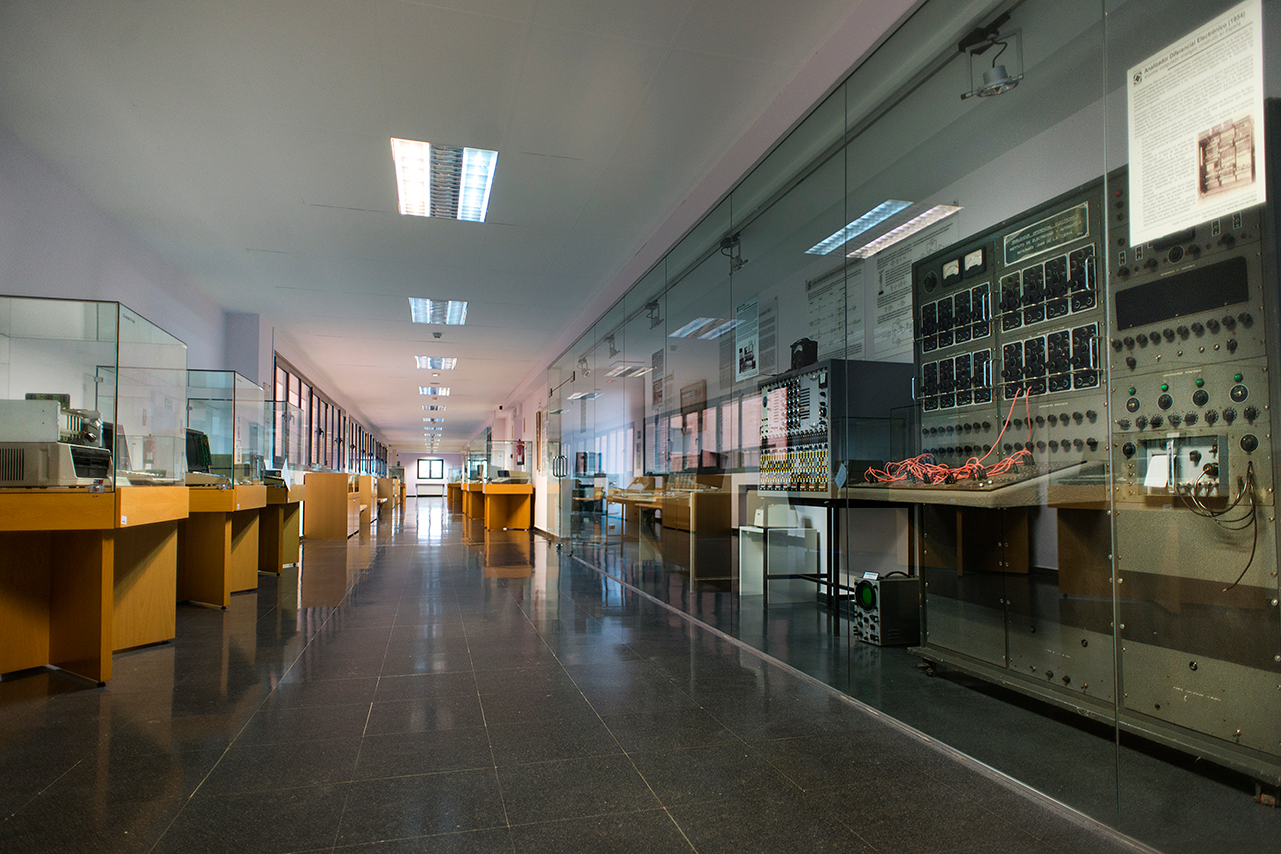
\includegraphics{images/image08.png}

Figura 1.1: Fotografía del museo

\begin{enumerate}
\setcounter{enumi}{2}
\item
  \hyperdef{}{h.3znysh7}{\subsection{Objetivos y
  motivación}\label{h.3znysh7}}
\end{enumerate}

~~~~~~~~Nuestro objetivo ha sido el desarrollo de una aplicación que
mejorará~la experiencia del usuario en un museo, en este caso, el museo
de la Facultad de Informática ``García-Santesmases''. Pero no solo esto,
sino que nuestro objetivo era hacerlo a través de los videojuegos y
utilizando la RA.

~~~~~~~~Esto lo logramos mediante una ``yincana'', guiando al visitante
a que recorra el museo en busca de misiones que tendrá que ir
completando minijuegos para poder pasar a la siguiente misión. Así, al
finalizar la visita, el jugador habrá recorrido el museo de una forma
amena y divertida.

~~~~~~~~Nuestra motivación principal en la realización de este proyecto,
fue profundizar en el desarrollo de videojuegos con una herramienta tan
innovadora como lo es la RA. Por lo que enseguida comenzamos a
investigar sobre aplicaciones creadas anteriormente y descubrimos que
los museos se están haciendo cada vez más eco de los beneficios de
aplicaciones como ésta para atraer al público. Esto nos motivó más, ya
que nos ponía delante una opción real de desarrollo.

\begin{enumerate}
\setcounter{enumi}{3}
\item
  \hyperdef{}{h.2et92p0}{\subsection{Antecedentes}\label{h.2et92p0}}
\end{enumerate}

~~~~~~~~El proyecto que hemos realizado para este TFG, es un proyecto
nuevo y que ha sido diseñado e implementado desde el principio por
nosotros. En años anteriores se realizaron trabajos de fin de grado
dedicados a la RA en museos, como el realizado el año pasado (2014/2015)
para el Museo de América. Nuestro proyecto guarda muchas similitudes con
el citado anteriormente, como el uso de RA en museos para mejorar la
experiencia del visitante. Por tanto, este trabajo puede que sea nuestro
antecedente, aunque el concepto de proyecto sea distinto, ya que ellos
utilizaban la RA como medio de información, mientras que nosotros
añadimos los videojuegos en RA como medio de entretenimiento en la
visita.

\begin{center}\rule{3in}{0.4pt}\end{center}

Capítulo 2:

Estado del arte

\begin{enumerate}
\item
  \hyperdef{}{h.3dy6vkm}{\subsection{La realidad
  aumentada}\label{h.3dy6vkm}}
\end{enumerate}

~~~~~~~~Según Ronald Azuma, desarrollador y líder de proyecto en New
Media,~Intel Corporation, y uno de los pioneros en el campo de la
realidad aumentada, dice que la RA consta de las siguientes
características:

\begin{itemize}
\itemsep1pt\parskip0pt\parsep0pt
\item
  Combina elementos reales y virtuales.
\item
  Es interactiva en tiempo real.
\item
  Está registrada en 3D.
\end{itemize}

A su vez, consta de unos requisitos mínimos para poder ser emulada, los
cuales son:

\begin{enumerate}
\itemsep1pt\parskip0pt\parsep0pt
\item
  Una pantalla, donde mostrar la combinación de los elementos reales
  captados por algún dispositivo y los elementos virtuales generados por
  un software.
\item
  Un conjunto de dispositivos que capturen los elementos del entorno~y
  nuestra situación como son una cámara, acelerómetro,
  giroscopio\ldots{} de tal forma que permita al software tener
  referencias de cómo y dónde debe mostrar sus elementos virtuales.
\item
  Un hardware relativamente potente, para poder realizar los cálculos
  necesarios para mostrar el entorno que captura la cámara y ser capaz
  de hacer frente al software que genera los elementos virtuales y
  combinarlos en la pantalla con los reales.
\item
  Un software capaz de reconocer el entorno y calcular donde y como debe
  representar los elementos virtuales combinados con los reales para
  conseguir una visión de RA.
\end{enumerate}

Con el continuo avance de los dispositivos móviles y la potencia, a un
coste aceptable para la mayoría, de la que constan ahora mismo estos,
permiten que cualquier usuario pueda hacer uso de la RA, ya que sus
Smartphones cumplen todos los requisitos para ello.

\begin{enumerate}
\setcounter{enumi}{1}
\item
  \hyperdef{}{h.1t3h5sf}{\subsection{Alcance}\label{h.1t3h5sf}}
\end{enumerate}

~~~~~~~~La RA es una tecnología que aunque ya lleva muchos años, no se
conocía a nivel usuario, pero el incremento tan alto del uso de los
Smartphones en los últimos años en la sociedad, ha permitido crear más
aplicaciones que todo el mundo pueda utilizar, ya que hoy en día casi
cualquier persona de una edad comprendida entre los 16 y 55 años tiene
un dispositivo móvil que le permite ejecutar una aplicación de RA en
cualquier lugar y momento.

~~~~~~~~Ahora mismo, tiene diferentes aplicaciones en diversos campos
como son:

\begin{enumerate}
\item
  \hyperdef{}{h.4d34og8}{\paragraph{Información
  interactiva}\label{h.4d34og8}}
\end{enumerate}

~~~~~~~~En este caso se utiliza para dar a conocer de forma interactiva
información acerca de un elemento cercano al usuario, de tal forma que
se puede mostrar un tipo de información u otra en función de la
interacción entre el usuario y dicho elemento.

~~~~~~~~Ahora mismo este área está muy presente en museos como forma
~dinámica de conseguir una inmersión del usuario con lo que está viendo
y hacer de su visita una experiencia más atractiva e incluso hasta más
productiva.

~~~~~~~~Dentro de este campo también se hace uso de la RA en
herramientas utilizadas para el intercambio de información en proyectos
profesionales o con fines comerciales como el de mostrar catálogos de
productos de una forma interactiva.
(http://ciencialaultima.blogspot.com.es/2015/01/realidad-aumentada-y-realidad-virtual.html)

\begin{enumerate}
\setcounter{enumi}{1}
\item
  \hyperdef{}{h.2s8eyo1}{\paragraph{Entretenimiento}\label{h.2s8eyo1}}
\end{enumerate}

~~~~~~~~En la actualidad, aunque no está todavía muy popularizado su
uso, existen una gran cantidad de videojuegos que hacen uso de esta
tecnología que, junto con diferentes mecánicas que se adaptan a ella,
generan una novedosa experiencia para entretener el usuario.

\begin{enumerate}
\setcounter{enumi}{2}
\item
  \hyperdef{}{h.17dp8vu}{\paragraph{Ciencia y
  desarrollo}\label{h.17dp8vu}}
\end{enumerate}

~~~~~~~~Aunque todavía no está normalizado el uso de la RA en este
campo, si están naciendo numerosos proyectos con el fin de desarrollar
esta tecnología para utilizarse en áreas como la medicina y la
construcción entre otras.
(http://mocadele.net/arloon-app-educativas-de-ciencias-con-realidad-aumentada/)

\begin{enumerate}
\setcounter{enumi}{3}
\item
  \hyperdef{}{h.3rdcrjn}{\paragraph{Otros}\label{h.3rdcrjn}}
\end{enumerate}

~~~~~~~~Además de los ya mencionados, existen todavía muchísimas áreas
en las que tienen cabida en sus tecnologías la RA además de muchos otros
usos que o bien están por descubrir o no se consta todavía de la
tecnología suficiente como para integrarlo.

Algo que todavía está en una fase temprana de desarrollo pero que tiene
un futuro prometedor es el uso de la RA para generación de terreno de
forma que se pueda reconocer el mismo y en función de su forma generar
un medio en relación un entorno que todavía no estaba registrado. Esta
tecnología dota de un sinfín de posibilidades añadidas a las ya
existentes para el uso de la RA en muchos otros campos.

2.3.~~~~~~~~Realidad Aumentada en videojuegos

~~~~~~~~La RA está siendo un gran descubrimiento para distintos ámbitos
en el mundo de la informática y la tecnología. Pero, el sector que más
interesado está en integrar la RA en sus desarrollos, para hacerla
llegar a gran parte de la sociedad, es el de los videojuegos.

En los últimos años, han aparecido nuevas formas de jugar, y todas ellas
intentan mejorar la experiencia del jugador, ya sea evadiendolo de la
realidad inventando un mundo y un espacio completamente nuevo, como hace
La Realidad Virtual, o como es en nuestro caso, añadiendo información al
mundo real, con la RA. Esta última consigue que el jugador maximice la
interacción con el juego, este motivo es lo que la hace tan atractiva
para la industria del videojuego.

~~~~~~~~

2.3.1 Ejemplos de Realidad Aumentada en videojuegos.

~~~~~~~~Hoy en día, la industria del videojuego está permanente
creciendo, y la competencia es tan grande que siempre se están buscando
nuevas formas de llamar la atención de los jugadores. Las nuevas
tecnologías como la Realidad Virtual o la Realidad Aumentada son de las
más utilizadas por las empresas para esto.

~~~~~~~~A continuación, se muestran algunos ejemplos de videojuegos con
RA.

\begin{itemize}
\itemsep1pt\parskip0pt\parsep0pt
\item
  Tarjetas RA Nintendo 3DS: Nintendo integra, desde su lanzamiento en
  2011, los juegos en RA en su nueva consola. Puedes jugar a distintos
  minijuegos, utilizando las 6 tarjetas AR Cards. El jugador tiene
  también la posibilidad de desbloquear nuevos minijuegos.
\end{itemize}

~~~~~~~~~~~~~~~~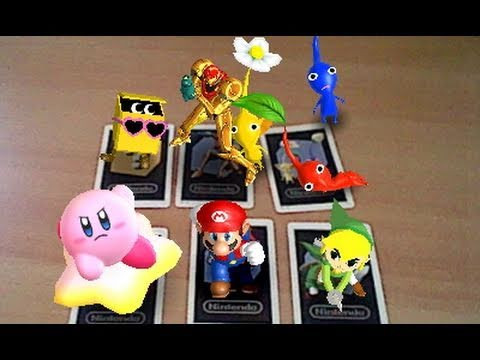
\includegraphics{images/image19.jpg}

~~~~~~~~~~~~~~~~A parte de estas aplicaciones preinstaladas en la
consola, Nintendo ha ido sacando distintos juegos que también utilizan
las AR Cards.

\begin{itemize}
\itemsep1pt\parskip0pt\parsep0pt
\item
  Pokémon Go: En esta versión, los jugadores podrán salir a explorar su
  ciudad e ir en busca de nuevos pokémon que se esconden por escenarios
  reales. Los encargados del desarrollo de este juego es la empresa
  Niantic Labs.
\end{itemize}

~~~~~~~~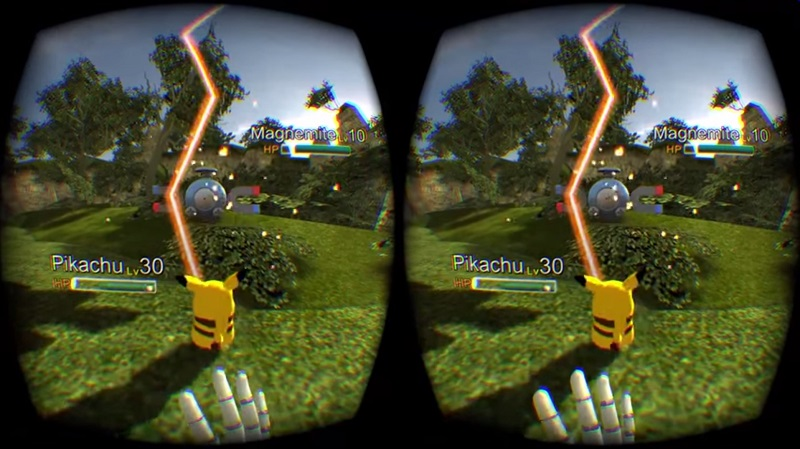
\includegraphics{images/image21.jpg}~~~~~~~~

\begin{itemize}
\itemsep1pt\parskip0pt\parsep0pt
\item
  Ingress: Este juego es otro ejemplo de desarrollo de Niantic Labs.
  Pero en esta ocasión, se trata de un juego de rol donde el jugador
\end{itemize}

~

2.4 Realidad Aumentada en Museos

~~~~~~~~La RA ha supuesto un avance muy importante en los museos ya que
aporta nuevas experiencias para los visitantes. Se usan diferentes
formas de usar la RA en el museo, desde aportar información adicional de
un objeto expuesto (enlace a un vídeo, descarga de contenido extra, más
información en texto, audios\ldots{}) hasta búsquedas del tesoro,
yincanas como la desarrollada en este trabajo\ldots{} todo ello son
experiencias añadidas y nuevas para la mayoría de museos.

A parte de los beneficios para el público, para el museo son formas de
añadir contenido muy baratas en relación con lo que puede costar hacer
obras para añadir salas, expositores\ldots{} Además, se puede añadir
contenido adicional a las aplicaciones, consiguiendo que el público
vuelva. Sí se puede contemplar la posibilidad de tener smartphones y/o
tabletas para el público visitante, una red WiFi abierta para facilitar
la descarga de la aplicación.

\subsection{2.4.1 El museo García Santesmases}\label{h.w6fqwheeko74}

~~~~~~~~Inaugurado en noviembre del 2003, el museo debe su nombre al
físico, profesor y precursor de la informática española José García
Santesmases, el cual fue catedrático de la Universidad Complutense. En
él, se exponen máquinas desarrolladas por la UCM entre 1970 y 1950.
Además, se exponen las computadoras comerciales del Centro de Cálculo de
la UCM, aportaciones de particulares, los propios departamentos de la
Universidad, etcétera.

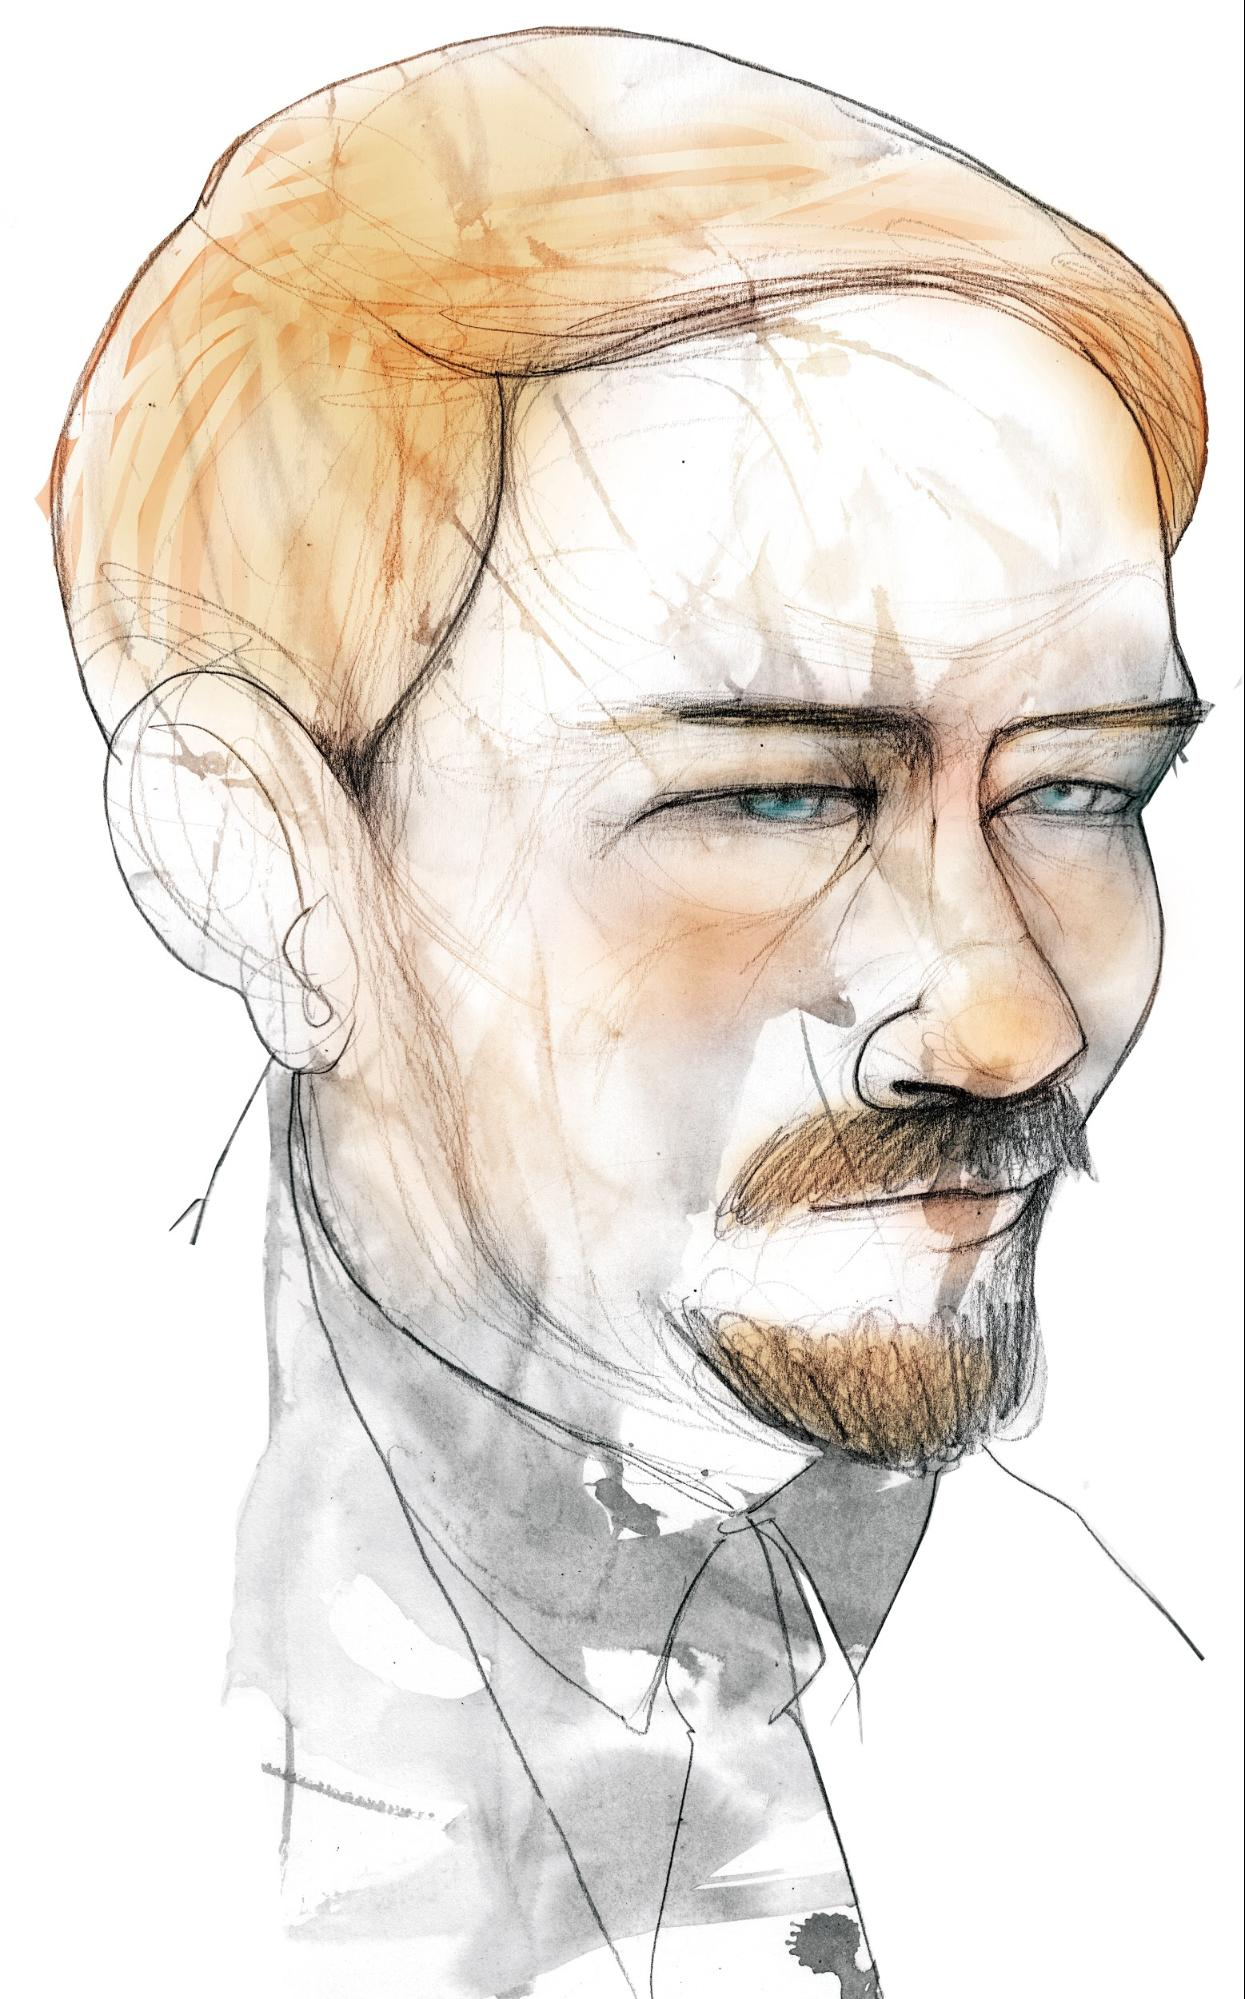
\includegraphics{images/image03.jpg}

~Retrato de José García Santesmases por Eulogia Merle

~~~~~~~~Además de computadoras, hay paneles explicativos que muestran
información sobre éstas y sobre historia de la informática en general y
cuenta también con gran cantidad de bibliografía presente en la
biblioteca de la facultad.

~~~~~~~~El museo cuenta con dos plantas situadas en la 3ª y 4ª planta de
la Facultad de Informática y su pieza más significativa es el
``Analizador diferencial electrónico'', diseñado por García Santesmases
y es el primer computador desarrollado en España.

\subsection{2.4.2 Otros museos}\label{h.alfq827rfehx}

~~~~~~~~Vamos a ver algunos de los museos que aplican la RA:

\begin{itemize}
\itemsep1pt\parskip0pt\parsep0pt
\item
  Centro de artes Ca l'Arenas del Museo de Mataró: para la exposición
  Mar de Fons el museo dispone de una aplicación que, al enfocar a
  cualquiera de los cuadros, se muestra información extra.
  ~\href{https://www.google.com/url?q=http://blogs.elpais.com/arte-en-la-edad-silicio/2012/05/construye-tu-propia-exhibicion.html\&sa=D\&ust=1464799690059000\&usg=AFQjCNEt_qw-SWuNUdtititu4dlhnNVyaw}{http://blogs.elpais.com/arte-en-la-edad-silicio/2012/05/construye-tu-propia-exhibicion.html}
\end{itemize}

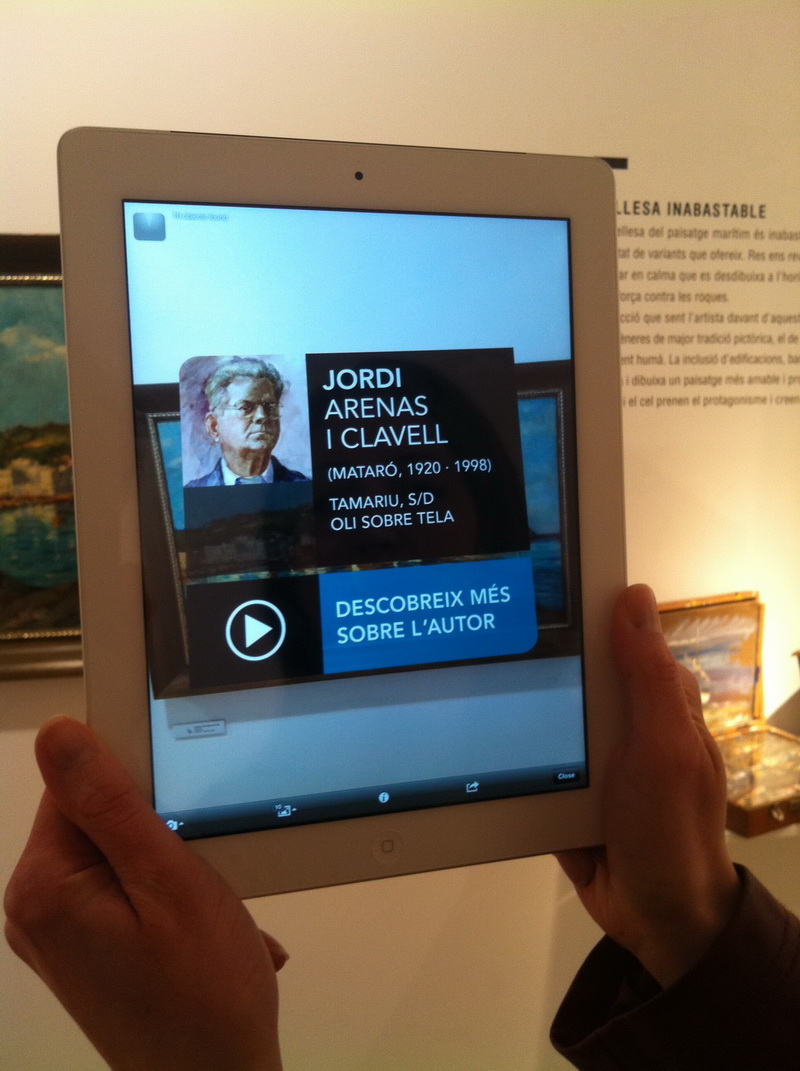
\includegraphics{images/image02.jpg}

Imagen 3.1: Aplicación del museo

\begin{itemize}
\itemsep1pt\parskip0pt\parsep0pt
\item
  Street Museum del Museo de Londres: una de las más famosas. Añade
  contenidos en el exterior del museo. Básicamente, nos permite ver
  fotografías antiguas de los sitios donde estamos, dándonos una visión
  de cómo era mientras vemos cómo es ahora ayudándose del
  posicionamiento GPS del dispositivo.
  \href{https://www.google.com/url?q=http://www.museumoflondon.org.uk/Resources/app/you-are-here-app/home.html\&sa=D\&ust=1464799690061000\&usg=AFQjCNHSmkQacw30ljnyv7J_7XluPlwZiw}{http://www.museumoflondon.org.uk/Resources/app/you-are-here-app/home.html}
\end{itemize}

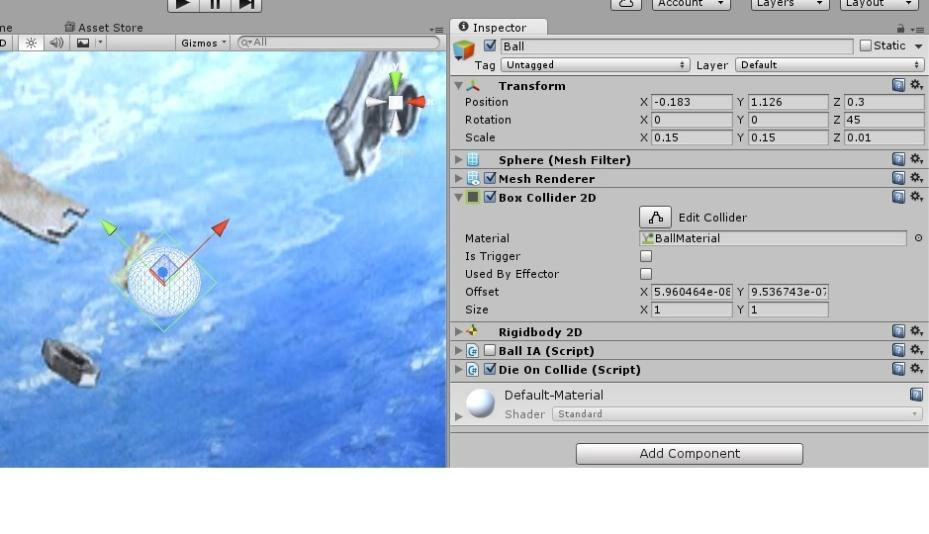
\includegraphics{images/image10.jpg}

Imagen 3.2: StreetMuseum (fuente
\href{https://www.google.com/url?q=http://www.noordtopics.nl/cultuur/2012_05_29-5.shtm\&sa=D\&ust=1464799690063000\&usg=AFQjCNE08rMhih_IPupKwcOaYUXUsWQkHw}{http://www.noordtopics.nl/cultuur/2012\_05\_29-5.shtm})

\begin{itemize}
\itemsep1pt\parskip0pt\parsep0pt
\item
  Crononautas del Museo Thyssen-Bornemisza de Madrid: esta aplicación
  pone al usuario como protagonista de una aventura con toques de
  ciencia ficción donde el usuario debe tomar decisiones que afectarán a
  la aventura. Además de servir de hilo conductor para la visita en el
  museo, aporta contenido adicional sobre las obras.
\end{itemize}

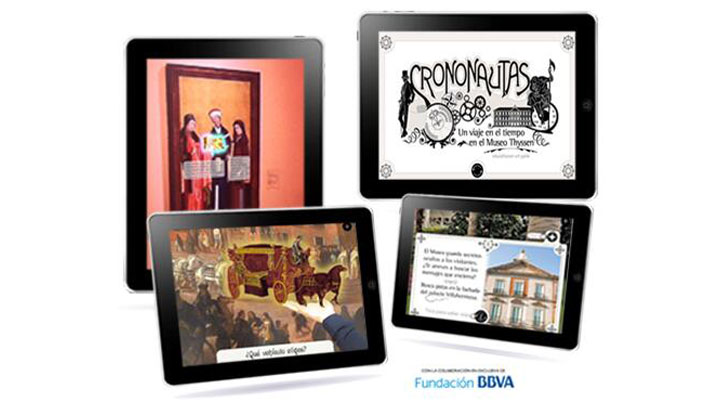
\includegraphics{images/image07.jpg}

Imagen: Crononautas

\begin{itemize}
\itemsep1pt\parskip0pt\parsep0pt
\item
  RACMA del Museo de América de Madrid: aplicación desarrollada por
  compañeros de esta misma facultad el curso pasado. En ella se ofrece
  información a los usuarios sobre distintas sociedades precolombinas.
  Además, nos muestra sobre un gran mapa mudo que se encuentra en el
  museo el lugar de influencia de varias de esas tribus y se puede
  interactuar con los personajes.
\end{itemize}

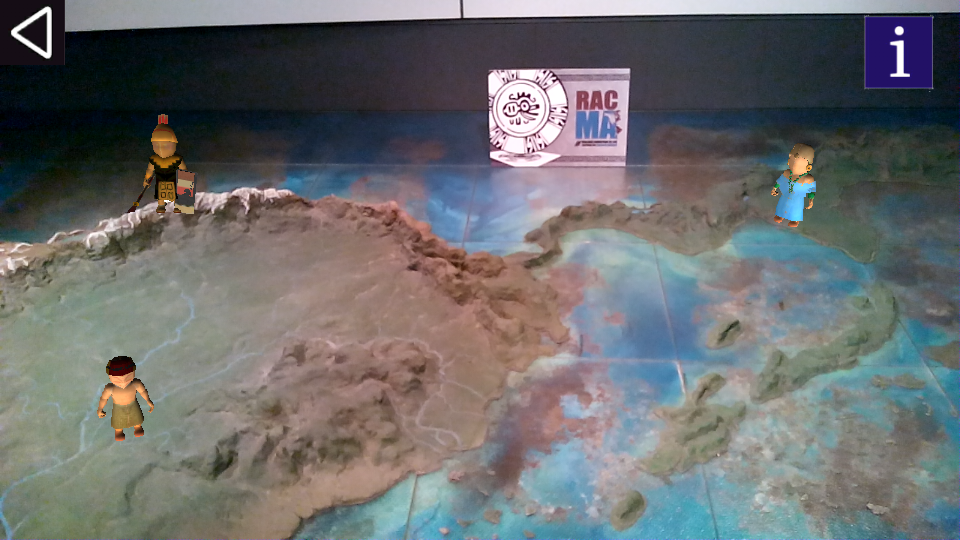
\includegraphics{images/image01.png}

Captura de RACMA que muestra las zonas de influencia de las sociedades
precolombinas.

\hyperdef{}{h.26in1rg}{\subsection{2.4.~~~~~~~~Herramientas de
desarrollo}\label{h.26in1rg}}

~~~~~~~~En este apartado explicaremos las herramientas que hemos
utilizado para la realización de este proyecto.

\hyperdef{}{h.lnxbz9}{\paragraph{2.3.1.~~~~~~~~Vuforia}\label{h.lnxbz9}}

Vuforia es el framework que hemos utilizado para hacer toda la parte de
RA. Es gratuito y tiene una gran comunidad, así como buenos ejemplos y
tutoriales. Facilita mucho el trabajo, y se puede utilizar con
diferentes SDK (Android, iOs, Unity 3D, ahora con gafas de realidad
virtual también\ldots{}).

\hyperdef{}{h.35nkun2}{\paragraph{2.3.2.~~~~~~~~Cómo generar realidad
aumentada}\label{h.35nkun2}}

~~~~~~~~Básicamente, Vuforia superpone a la imagen tomada por la cámara
de, en este caso, nuestro Smartphone, cualquier modelo en tres
dimensiones que queramos sobre la posición de un~Image Target~(u otro
marcador) que le hayamos indicado. De esta manera, tenemos un ``fondo''
con la imagen tomada por la cámara, con modelos en tres dimensiones
``por encima''. Además, nos mantiene siempre los objetos de tres
dimensiones en el mismo punto del espacio, por lo que si movemos nuestra
cámara, cambiará la perspectiva desde donde vemos el objeto, pudiendo
girar alrededor de éste. El comportamiento puede ser diferente,
dependiendo de cómo lo hayamos configurado (podemos hacer que el objeto
persista aun que perdamos de vista el detector).

\hyperdef{}{h.1ksv4uv}{\paragraph{2.3.3.~~~~~~~~Plataformas de
desarrollo}\label{h.1ksv4uv}}

~~~~~~~~Vuforia proporciona paquetes para trabajar directamente con el
SDK de Android o el de iOS, así como para Unity3D. Utilizando Unity3D
podemos exportarlo después a una aplicación de Android o iOS también,
aunque no quedaría de una manera tan ``pulida'' como desarrollándola
directamente con el SDK del sistema operativo deseado. Nosotros hemos
decidido utilizar el paquete para Unity3D porque los tres teníamos unos
conocimientos básicos en desarrollo con Unity, además de que nos permite
exportar después el proyecto al sistema operativo que quisiéramos.

\hyperdef{}{h.44sinio}{\paragraph{Unity}\label{h.44sinio}}

Unity funciona con algo a lo que han llamado~escenas, que son diferentes
situaciones o niveles del juego. En toda escena hay una jerarquía de
objetos que la componen, y de cada objeto pueden~colgar~otros objetos,
además de que se pueden añadir (por medio de código programable) otros
objetos a esa jerarquía de manera dinámica. Todos los objetos de Unity
tienen una serie de componentes, el más básico sería el de su situación
en las tres dimensiones (o dos), su escala y su rotación con respecto a
los tres planos. Estos componentes permiten configurar los objetos de
manera sencilla, encapsulando funcionalidades. Esta forma de
``componer'' los objetos no es casual: es la más utilizada en
programación de videojuegos. (ejemplo
http://forum.unity3d.com/attachments/screen-shot-2014-05-27-at-2-34-04-pm-png.102002/)

~~~~~~~~Además, Unity cuenta con una extensísima comunidad de
desarrolladores, así como tutoriales, guías, dudas resueltas\ldots{}
solo con los tutoriales que proporciona la propia gente de Unity podemos
hacer un sencillo juego casi de cada uno de los tipos más comunes de
juegos.

~~~~~~~~Unity nos proporciona por defecto el cálculo de colisiones entre
objetos, gravedad, eventos de teclado o ratón\ldots{} en pocos minutos
podemos hacer cosas sencillas pero que con otras herramientas, o
programándolo directamente a mano con un lenguaje de programación
cualquiera como podría ser Java o C++, nos llevarían bastante más
tiempo.

\paragraph{}\label{h.sl0g53rzcit}

\hyperdef{}{h.2jxsxqh}{\paragraph{C\#}\label{h.2jxsxqh}}

~~~~~~~~Los~scripts~los podemos escribir en C\#, Boo o un lenguaje
``parecido'' a JavaScript. Nosotros hemos decidido utilizar C\#, ya que
era la opción que más nos convencía por varias razones:

\begin{itemize}
\itemsep1pt\parskip0pt\parsep0pt
\item
  Hemos leído que es más eficiente.
  {[}\href{https://www.google.com/url?q=http://answers.unity3d.com/questions/7567/is-there-a-performance-difference-between-unitys-j.html\&sa=D\&ust=1464799690077000\&usg=AFQjCNGmmgnF39Uu5qMADlO87GMttS0Q5Q}{http://answers.unity3d.com/questions/7567/is-there-a-performance-difference-between-unitys-j.html}{]}
\item
  Los tres teníamos conocimientos previos de Java, y C\# es muy similar
  a Java en cuanto a sintaxis.
\item
  Es el más usado por la comunidad.
  {[}\href{https://www.google.com/url?q=http://forum.unity3d.com/threads/boo-c-and-javascript-in-unity-experiences-and-opinions.18507/\&sa=D\&ust=1464799690080000\&usg=AFQjCNESW4HtOPW0LsIGsCR-C3rJQjk-YA}{http://forum.unity3d.com/threads/boo-c-and-javascript-in-unity-experiences-and-opinions.18507/}{]}
\end{itemize}

~~~~~~~~Todos los~Scripts~utilizados en Unity heredan de la
clase~MonoBehaviour, la cual permite a estos~scripts~integrarse con la
ejecución interna de Unity. Toda clase que herede de MonoBehaviour~tiene
los métodos Start (), Awake (), Update (), FixedUpdate (), y OnGUI (),
entre otros.

~~~~~~~~Éstos se ejecutan en diferentes momentos del juego.

\begin{enumerate}
\itemsep1pt\parskip0pt\parsep0pt
\item
  Awake (): el primer método al que se llama, antes incluso de que el
  objeto asociado esté habilitado en la escena. Se utiliza para
  inicializaciones o referencias entre~scripts.
\item
  Start (): se ejecuta después de~Awake (), justo antes del
  primer~Update ()~y después de que se active el objeto.
\item
  Update (): se ejecuta en cada~frame. Esto hace que dependa del
  procesador y del equipo donde se ejecuta. Se usa para actualizaciones
  comunes como mover objetos no físicos, recoger entrada del
  usuario\ldots{}
\item
  FixedUpdate (): el intervalo entre una ejecución y otra es consistente
  y siempre el mismo. Se utiliza para actualizaciones como ajustar
  objetos físicos.
\item
  OnGUI (): se utiliza para gestionar y renderizar eventos de
  la~Interfaz Gráfica de Usuario~(Graphic User Interface,~GUI). Sólo es
  llamada si el objeto está habilitado.
\end{enumerate}

\subsection{~~~~~~~~}

\hyperdef{}{h.z337ya}{\paragraph{Unity + Vuforia}\label{h.z337ya}}

~~~~~~~~Vuforia nos proporciona un paquete de extensión de Unity 3D el
cual debemos importar para trabajar. Éste paquete contiene
diferentes~prefabs~(objetos ya construidos) que nos harán la tarea muy
sencilla.

~~~~~~~~Lo que debe tener toda aplicación de RA hecha con Vuforia y
Unity 3D es una ARCamera (cámara de RA). A ésta hay que indicarle
el~product key~que nos da Vuforia desde su portal para desarrolladores,
además de ésto, se le indicará el paquete de targets~propios (lo
explicaremos más adelante en profundidad). Es la unidad mínima de
desarrollo de RA con Vuforia.

~~~~~~~~Una vez hecho esto, tendremos diferentes opciones para lanzar
los objetos de RA, que deben colgar en la jerarquía de Unity de
cualquiera de los siguientes~prefabs:

\begin{enumerate}
\itemsep1pt\parskip0pt\parsep0pt
\item
  Frame Markers:
\end{enumerate}

Son marcadores muy sencillos que son proporcionados por la gente de
Vuforia en su paquete. Se pueden utilizar para calibrar la cámara, pero
no tienen una gran calidad a la hora de ser detectados. Son lo más
sencillo para comenzar una aplicación de prueba.

\begin{enumerate}
\setcounter{enumi}{1}
\itemsep1pt\parskip0pt\parsep0pt
\item
  Image Targets:
\end{enumerate}

Imágenes propias del desarrollador. Funcionan como los Frame Markers,
pero éstas deben ser importadas desde un paquete generado por el portal
de desarrolladores de Vuforia, el cual nos indicará la calidad de esa
imagen para ser detectada.

~~~~~~~~~~~~~~~~~ ~~~~~~~~~~~~~~~~~

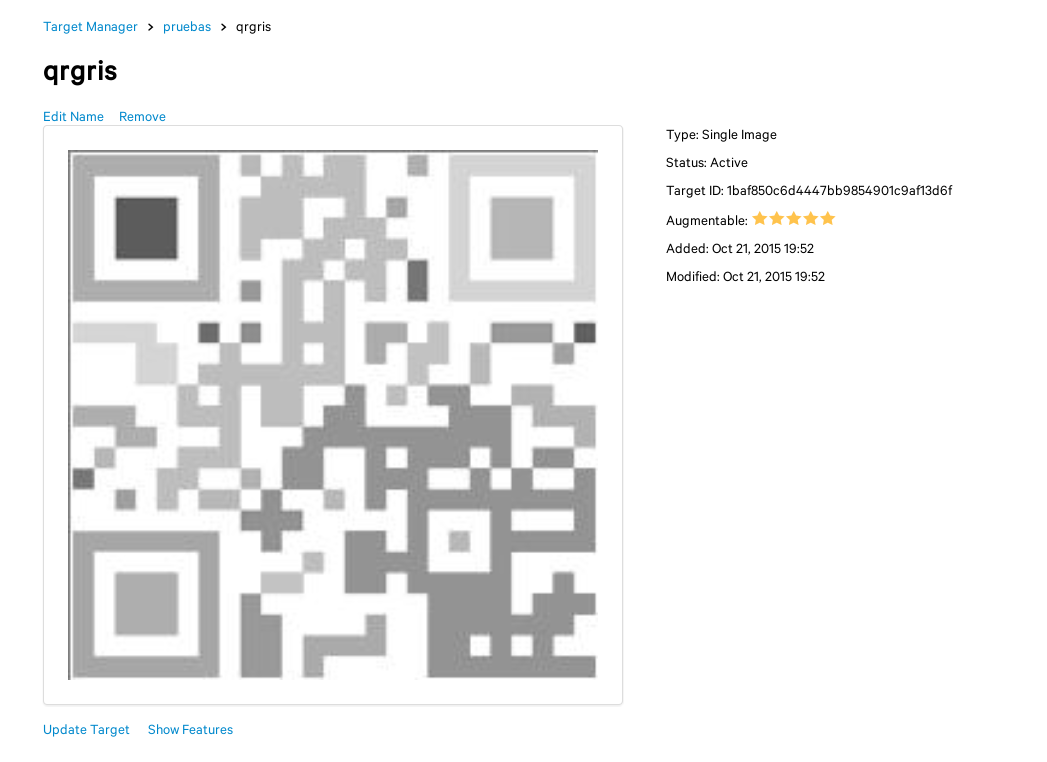
\includegraphics{images/image11.png}

Figura5: Ejemplo de calidad de un ImageTarget en la plataforma para
desarrolladores de Vuforia

\begin{enumerate}
\setcounter{enumi}{2}
\itemsep1pt\parskip0pt\parsep0pt
\item
  Multi-Targets:
\end{enumerate}

Son varios~ImageTargets~que representan las diferentes caras de un
prisma en tres dimensiones.

\begin{enumerate}
\setcounter{enumi}{3}
\itemsep1pt\parskip0pt\parsep0pt
\item
  Cylinder Targets:~
\end{enumerate}

ImageTarget~que envuelve un cilindro, para representar, por ejemplo, una
botella u otro objeto similar.

\begin{enumerate}
\setcounter{enumi}{4}
\itemsep1pt\parskip0pt\parsep0pt
\item
  Text Recognition:
\end{enumerate}

Nos permite detectar textos, ya sean del diccionario proporcionado por
Vuforia de palabras en inglés (más de 100.000 palabras diferentes) o de
uno creado por nosotros mismos.

\begin{enumerate}
\setcounter{enumi}{5}
\itemsep1pt\parskip0pt\parsep0pt
\item
  Object Recognition:
\end{enumerate}

Sirve para configurar un objeto en tres dimensiones que no sea ninguno
de los anteriores.

\begin{enumerate}
\setcounter{enumi}{6}
\itemsep1pt\parskip0pt\parsep0pt
\item
  Smart Terrain:
\end{enumerate}

Permite reconstruir el entorno del usuario de la aplicación en tres
dimensiones. ~~~~~~~~~~~~~~~~~ ~~~~~~~~

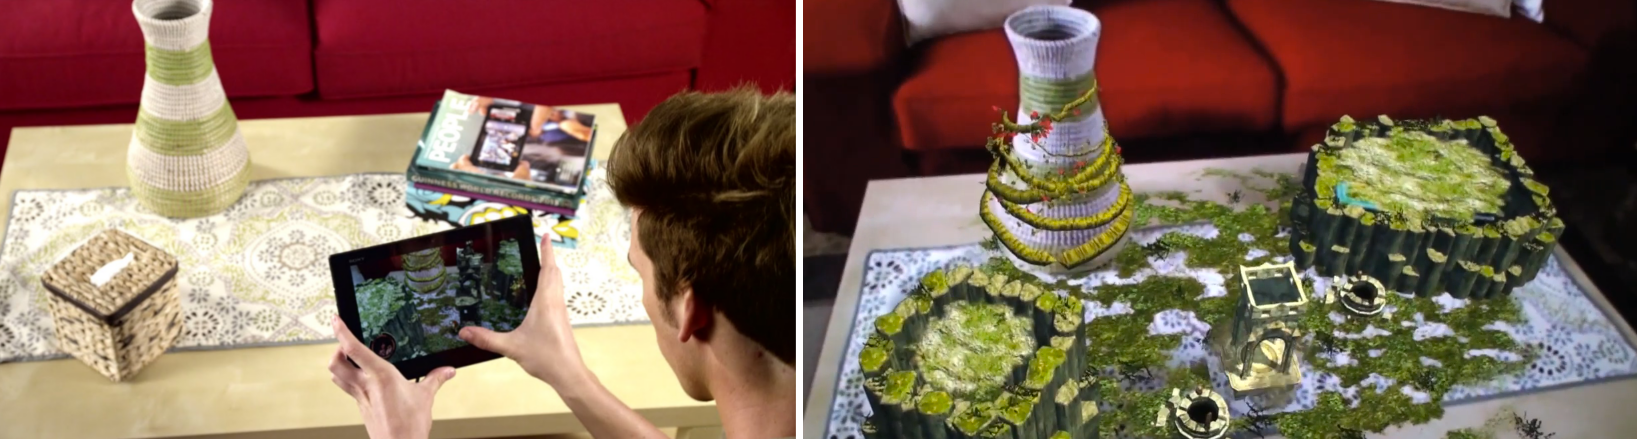
\includegraphics{images/image13.png}

Figura 3: Ejemplo de aplicación con Smart Terrain

Con cualquiera de estos objetos, la funcionalidad por defecto (que
podemos modificar creando nuestras propias clases que hereden de las que
nos da Vuforia) es que al detectarse (ya sea un ImageTarget, un Text
Recognition, etcétera) se comenzarán a mostrar todos los objetos que
cuelguen de él en la jerarquía de Unity.

~~~~~~~~

\begin{center}\rule{3in}{0.4pt}\end{center}

Capítulo 4:

Diseño del videojuego

\subsection{4.1.~~~~~~~~Introducción}

~~~~~~~~El trabajo que se ha realizado para este proyecto es un
videojuego. Éste está ambientado en el espacio y hace uso de la RA como
entorno.

La idea principal del proyecto es la de implementar minijuegos con
diferentes mecánicas y adaptarlos a su uso con RA y la tecnología móvil.
Con este fin, creemos que se puede hacer de cualquier espacio un lugar
mucho más interesante haciendo uso de esta tecnología, ya que no solo
imaginas la realidad del lugar sino que puedes interactuar con
él.~~~~~~~~

Con el fin de hacer uso de la tecnología actual que se nos brinda para
el desarrollo de la RA, hemos implementado tres juegos que creíamos
viables, y que nos permiten poder experimentar con ella. Estos tres
juegos son un Space invaders adaptado al uso de la RA, el Arkanoid~y
WaterPipes. Los tres, están unidos haciendo uso de un hilo argumental
que no solo da coherencia a los juegos, sino que obliga al usuario a
moverse por la facultad para poder completar los niveles.

\hyperdef{}{h.4i7ojhp}{\subsection{4.2.~~~~~~~~Hilo
argumental}\label{h.4i7ojhp}}

El videojuego nos traslada a una nave espacial que está siendo atacada
por unos alienígenas. El piloto de la nave nos pondrá en situación y nos
irá pidiendo que realicemos diferentes tareas para que la nave pueda
despegar. De ésta forma conseguimos que el jugador se mueva por
diferentes sitios del museo, ya que a cada minijuego solo se puede jugar
en un punto del museo. Así añadimos dinamismo a la aplicación. Además,
hay un sistema de puntuación diferente para cada minijuego y solo una
oportunidad para cada minijuego.

Al principio nos pedirá que destruyamos a los alienígenas que nos están
atacando. Para ello, debemos salir al exterior de la nave (la puerta de
entrada de la facultad), donde comienza el primer minijuego al enfocar
el cartel de la Facultad de Informática. Así, comenzamos a jugar al
Space Invaders. Conseguiremos puntos cada vez que destruyamos un
invasor, y perderemos puntos si no conseguimos destruir todos antes de
que destruyan el escudo de la nave.

A continuación, el piloto nos pedirá que limpiemos los restos de las
naves invasoras. Para ésto debemos ir a los mandos del robot de
reciclaje (la máquina arcade que hay en la tercera planta del museo) y
así comenzará el segundo minijuego, el Arkanoid. En este conseguimos
puntos cuando la bola choca contra la ``chatarra espacial''.

Por último, libres de enemigos y con el camino despejado, solo nos queda
un escollo para poder escapar. ~Los tubos del sistema de propulsión por
los que va el combustible no están bien alineados y tenemos que rehacer
el camino desde el depósito hasta el motor. Para ésto debemos ir al
puesto de mando donde está el panel informativo del sistema de
combustión (cartel ``Simulador Básico de Centrales térmicas'' del otro
pasillo de la tercera planta) y reajustarlos. Aquí comienza el tercer y
último minijuego, WaterPipes. Éste minijuego va por tiempo, y debemos
encontrar un camino para el combustible antes de que se agote. La
puntuación, con este minijuego, solo puede disminuir, pero en nuestra
mano está que el camino sea lo más corto posible y así se nos reste el
mínimo posible de puntos.

Al finalizar, nuestra tarea habrá acabado. Se nos pedirá que
introduzcamos nuestro nombre, y este se añadirá a un ``Hall de la fama''
de todos los usuarios del juego, ordenados por puntuación. Con ésto,
hemos querido intentar que el juego sea rejugable por los usuarios, que
intentarán conseguir más puntos afinando su puntería o su velocidad para
quedar más alto del ``Hall de la fama''.

~~~~~~~~

YO BORRARÍA TODO DESDE AQUÍ\ldots{}

Inicialmente nos reunimos para definir nuestros objetivos para este
proyecto y así posteriormente diseñar un primer boceto de lo que será
nuestra aplicación. Como la idea fundamental del proyecto está bastante
clara, realizar una aplicación con varios mini juegos por el museo
``García-Santesmases'' de la facultad, con RA; decidimos investigar qué
tipo de juegos podemos implementar, para ello realizaremos un estudio de
los juegos ya existentes en museos con y sin RA, e iremos al museo de la
facultad. Durante la visita al museo, y ya con una idea de lo que
podemos o no desarrollar, obtendremos una lista de los posibles juegos
que podemos realizar en distintas partes del museo.

~~~~~~~~Una vez elegidos los juegos, haremos un pequeño estudio del
alcance del proyecto y decidiremos cuales son los juegos más viables,
teniendo en cuenta el tiempo de desarrollo y pero sobretodo la
experiencia del usuario. Aunque la aplicación se basa en varios
minijuegos repartidos por diferentes zonas del museo, no hay que olvidar
que el objetivo principal es mejorar la experiencia del usuario y para
conseguirlo es fundamental crear un hilo argumentativo que facilite al
usuario encontrar los juegos y lo más importante añada emoción y
diversión a la visita. Por lo que, cuando ya tengamos los juegos y
sepamos la distribución por el museo, debemos crear un hilo argumental
que una de una manera amena todos los juegos entre sí. Cuando tengamos
una versión estable, realizaremos pruebas con usuarios de distintos
perfiles, para poder obtener un estudio de viabilidad de la aplicación
más fiable y detallada.

\subsection{4.3 Otros aspectos}\label{h.yyppnqmy8a9a}

\subsection{ESCENAS INTERMEDIAS}\label{h.hulp4wa8ygn2}

Entre cada escena; o minijuego del desarrollo, se ha establecido una
intermedia donde un ``humanoide'' nos pone en situación antes de cada
misión y nos sitúa acerca de cómo se ha llegado a dicha situación y a
dónde debemos ir para resolverla.

\includegraphics{images/image00.png}

Figura X.Y: Diagrama de flujo entre las escenas del juego (hecho con
draw.io)

Gracias al paquete de Unity animación por voz, SAMBA, el proceso de
sincronizar el audio con la animación del discurso del modelo ha sido
algo muy sencillo. Dicha animación consta de tres componentes:

\begin{enumerate}
\itemsep1pt\parskip0pt\parsep0pt
\item
  El modelo, que en este caso era un prefab~que venía configurado por
  defecto para soportar el componente de audio y de enfoque aleatoria.
\item
  Componente de animación de los músculos faciales, al cual se le asigna
  un conjunto de audios de tal forma que la cara del modelo se articula
  de forma sincronizada con el audio proporcionado. El componente viene
  configurado para que el audio que le proporcionamos al modelo pueda
  ser interpretado por este con más o menos énfasis o con diferentes
  estados de ánimo.
\item
  Random eyes~es un componente que, asignado al modelo, articula sus
  ojos de tal forma que definiendo unos puntos objetivo, alterna y
  gesticula mirando a los diferentes objetivos a lo largo de la
  animación del objeto.
\end{enumerate}

Además del modelo utilizado, también hubo que crear los audios que
narran el hilo argumental de nuestro juego. Para esta tarea, se
generarón los audio con la herramienta de la url
\href{https://www.google.com/url?q=http://vozme.com/index.php?lang\%3Des\&sa=D\&ust=1464799690122000\&usg=AFQjCNHd3r7Z3_MhdyjbXYSTkEUQQ8dnZg}{http://vozme.com/index.php?lang=es}~que
convierte a *.mp3, con una voz un ``robótica'', un texto dado.

En último lugar, la escena contiene también un texto donde se muestra de
forma escrita todo lo que se va narrando. Esto es así porque pueden
haber problemas de audio, o el usuario puede tener la necesidad de
volver a ver el mensaje y sintetizar lo que el ``robot'' ha dicho para
poder encontrar el próximo lugar donde aparecerá el siguiente minijuego.

{[}imagen de una escena intermedia{]}

\subsection{SISTEMA DE PERSISTENCIA DE
PUNTUACIONES}\label{h.es5w8jt0xlk6}

Al finalizar el juego, el usuario puede almacenar su puntuación, y ver
el ranking de estas. Este sistema se hizo para enlazar el juego con lo
que es un servicio web, ya que nos parecía una práctica interesante el
hacer uso de la parte cliente que nos ofrece Unity para comunicarnos con
servicios web. ;Se han implementado ambas partes en este caso, tanto el
lado cliente que consume los servicios en Unity, como el lado del
servidor, en el que se ha implementado un sistema de gestión de usuarios
con una sencilla api REST en PHP, haciendo uso del framework Symfony 2.

Desarrollo

Diseño

\begin{itemize}
\itemsep1pt\parskip0pt\parsep0pt
\item
  Base de datos: Se genera una base de datos SQL con una sola tabla, la
  de usuarios y los campos que deseábamos guardar: id, nombre y
  puntuación.
\item
  {[}imagen de phpMyAdmin tabla de usuarios{]}
\item
  Operaciones: Para la parte REST; los servicios, solo pueden realizar
  las operaciones de leer y crear nuevos usuarios. En el panel de
  administración, se pueden realizar las CRUD, crear un nuevo usuario,
  leer los usuarios y ver el usuario en detalle, actualizar y eliminar.
\item
  Panel de administración: Se accede con el usuario administrador a
  través de la siguiente URL
  \href{https://www.google.com/url?q=http://augmentedreality.hol.es/web/users/\&sa=D\&ust=1464799690127000\&usg=AFQjCNGoTkjRzj7Cigk_Eycmo5Kp9tVzyA}{http://augmentedreality.hol.es/web/users/}~y
  en ella se pueden realizar las descritas en el apartado anterior.
\item
  REST: la URL base es
  \href{https://www.google.com/url?q=http://augmentedreality.hol.es/api/\&sa=D\&ust=1464799690128000\&usg=AFQjCNHy0MPDl_4cBnnxwHjLI1fgilZRmg}{http://augmentedreality.hol.es/api/}~y
  las operaciones son; de tipo GET~/users.{[}json \textbar{} xml{]} para
  obtener un listado de los usuarios y sus puntuaciones en uno de los
  formatos especificados. Y para guardar la puntuación de un usuario, de
  tipo POST~/api/users dónde se les manda, en el body de la petición, la
  puntuación del usuario y el nombre de este.
\item
  Seguridad: De lado del servidor, Symfony~nos provee de un sistema de
  seguridad basado en tres factores; la dirección a la que se accede, la
  autenticación para acceder a ella y una vez autenticado, el rol que
  tiene dicho usuario para poder acceder. En nuestro caso hay dos
  usuario. ``admin'', con el rol de administrador, que le permite entrar
  tanto en el panel de administración, como hacer uso de la api. Y
  ``api\_user'', un usuario cuyo rol solo le permite usar los servicios
  web. El tipo de autenticación es a través de Basic auth. Consiste en
  añadir un campo en el header~con la clave ``Authorization'' y como
  valor, la palabra ``Basic'' concatenada y separados por un espacio con
  la combinación de ``username:password'' codificada en Base64.
\end{itemize}

HASTA AQUI

\subsection{4.3.~~~~~~~~Conclusiones}

~~~~~~~~En general hemos quedado bastante satisfechos con el resultado
final. Sí nos hemos dado cuenta que podríamos haber implementado más
minijuegos, pero los primeros meses fueron bastante lentos en cuanto a
desarrollo.

~~~~~~~~Creemos que la yimcana es una buena manera para que el usuario
del museo se mueva por éste.

FUERA\ldots{}.

Fuimos probando las diferentes técnicas individualmente y aprendiendo
Unity3D según la necesidad de cada uno. Además, la RA y la librería de
Vuforia nos dieron algunos problemas que explicamos con más detalle en
los siguientes capítulos que no esperábamos, por lo que el tiempo que en
un principio consideramos que nos iba a llevar fue mayor.

Hemos visto que es bastante interesante tanto la RA en museos como los
videojuegos con RA. Además, al hacer versiones de juegos clásicos, hemos
podido intentar darle un vuelto a las mecánicas y una visión nueva. Si
ya de por si la RA en museos es un gran atractivo para acercar al
público jóven a los museos, con la inclusión de minijuegos (que no tenga
partidas largas) creemos que es algo con un gran potencial a explotar.

Sí que hemos visto que la interacción con el Smartphone es algo a
revisar, ya que interactuar con el móvil mientras se apunta en una
dirección en particular puede ser incómodo si hay que hacer pulsaciones
en diferentes puntos de la pantalla.

..HASTA AQUÍ

\begin{center}\rule{3in}{0.4pt}\end{center}

Capítulo 5:

Space Invaders

\begin{enumerate}
\item
  \hyperdef{}{h.3whwml4}{\subsection{Historia}\label{h.3whwml4}}
\end{enumerate}

~~~~~~~~Quizá uno de los juegos~arcade~clásicos más conocidos. La
primera versión salió al mercado en 1978, hace casi cuarenta años. Uno
de los precursores del género~shoot 'em up. El jugador controla una nave
espacial que se mueve horizontalmente y debe hacer frente a~hordas~de
alienígenas enemigos que atacan al jugador disparándole proyectiles.
Además, a veces el jugador cuenta con pequeñas construcciones que hacen
la labor de~búnker~donde ponerse a cubierto de los disparos, aunque
éstos se van destruyendo.

~~~~~~~~~~~~~~~~~ ~~~~~~~~~~~~~~~~~

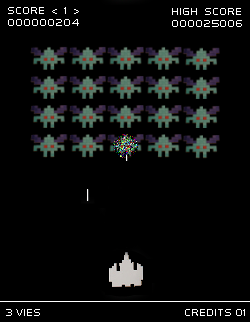
\includegraphics{images/image12.png}

Figura 4: Space Invader original

Éste juego está ampliamente extendido en la cultura popular ya que es
uno de los grandes clásicos, por eso hemos considerado acertado
incluirlo en nuestro proyecto.

~~~~~~~~

\begin{enumerate}
\setcounter{enumi}{1}
\item
  \hyperdef{}{h.2bn6wsx}{\subsection{Nuestra versión}\label{h.2bn6wsx}}
\end{enumerate}

~~~~~~~~Nosotros hemos decidido darle un cambio a la jugabilidad del
juego, y cambiar el sistema. En nuestra versión utilizamos la RA para
que la experiencia sea completamente diferente. Nuestro juego arrancará
al detectar el cartel de~FACULTAD DE INFORMÁTICA~(Text Recognition),
mostrándonos unos invasores alienígenas sobre el cartel, y
unas~defensas~bajo éste.

{[}imagen de como empieza el juego en el cartel de la facultad{]}

Para destruir a los invasores, lo que tenemos que hacer es mover
nuestro~Smartphone~para mover nuestra cámara y pulsar en la pantalla
para realizar el disparo. Hemos pasado de manejar la nave defensora en
tercera persona, a hacerlo en primera persona, con un punto de mira en
el centro de la pantalla que nos marca en qué dirección irán los láseres
de nuestra~torreta de defensa, convirtiendo el juego en un~First Person
Shooter, y tendremos que hacerlo antes de que los enemigos consigan
destruir el escudo de nuestra nave espacial (cuando pasa del verde al
rojo). Iremos obteniendo puntos según destruyamos naves enemigas, y
perderemos puntos al recibir impactos en el escudo, por lo que cuanto
más rápidos seamos, más puntos obtendremos.

Con estos cambios, hemos conseguido (a nuestro juicio), transformar un
clásico de los~arcade~en un nuevo juego que utiliza la RA dando una
experiencia diferente.

\begin{enumerate}
\setcounter{enumi}{2}
\item
  \hyperdef{}{h.qsh70q}{\subsection{Implementación}\label{h.qsh70q}}
\end{enumerate}

~~~~~~~~Durante el desarrollo de este juego hemos encontrado unos
cuantos escollos que superar, algunos que nos han llevado quebraderos de
cabeza. Comenzamos desarrollando el videojuego utilizando un código QR
como~marcador~de la RA, pensando que después pasar a utilizar un texto
no tendría complicaciones. Una vez teníamos el juego desarrollado con un
código QR (ImageTarget), probamos a detectar texto propio, ya que
Vuforia nos da un diccionario con miles de palabras en inglés, pero
nosotros no queríamos detectar esas palabras, si no únicamente~FACULTAD
DE INFORMÁTICA.

~~~~~~~~Para esto, seguimos los tutoriales de Vuforia, y, tras resolver
algunas dudas, implementamos una escena sencilla en la que se mostraba
una esfera sobre el texto. Después, intentamos transferir lo
desarrollado con el~ImageTarget, al texto.

~~~~~~~~Entonces surgieron los problemas. El primero que vimos, era que
las proporciones de nuestros~Invasores~y las~Defensas~se quedaron muy
pequeñas, haciendo imposible jugar cómodamente. La mejor manera que
conseguimos para que se ajustaran los elementos del juego a un tamaño
aceptable fue mediante un Script de C\# que aumentaba la escala local de
los Invasores~y las Defensas~(local scale).

~~~~~~~~El siguiente problema que encontramos fue al~insertar~nuestro
Enjambre de~Invasores. Por un lado, una vez aparecían los enemigos, si
movíamos la cámara, éstos se quedaban en la misma posición respecto a la
cámara, es decir, si cuando salían por primera vez estaban en la parte
superior izquierda (por ejemplo) de la pantalla, y nos movíamos, seguían
ahí, en vez de ajustar su posición con respecto al texto detectado.
Tuvimos que cambiar la forma en la que los insertábamos en la escena,
antes de manera dinámica y creando una instancia con un Script, y ahora
como hijos del~GameObject~que representa al texto detectado. Éste tipo
de problema (de la posición respecto a los objetos de RA) nos volvería a
salir más adelante, pero con los proyectiles que lanzábamos para acabar
con los enemigos.

~~~~~~~~En las primeras versiones del juego, lanzábamos un prisma
(nuestro~Proyectil) contra los enemigos. Según lanzábamos, el proyectil
se iba dirigiendo en la dirección que tenía la cámara respecto
al~ImageTarget~al realizar el disparo. Al pasar a utilizar el texto,
esto cambió. Vimos que nuestro disparo se mantenía siempre en el vector
de dirección de la cámara, y cambiaba con éste. Es decir, nuestro
proyectil~siempre~estaba en el centro de la pantalla, con lo cual se
perdía toda la gracia al juego y su jugabilidad pasaba a ser bastante
complicada. Éste problema nos dejó bastante confusos, ya que con cambiar
el objeto de la RA (ImageTarget~o TextRecognition) cambiaba el
comportamiento del proyectil.

~~~~~~~~Para resolver esto, cambiamos nuestro proyectil por un~láser.
Ahora al tocar la pantalla no se~lanza~un proyectil, si no que se
dispara un~láser~que destruirá los enemigos que estén en el vector de
dirección de la cámara. Así hemos conseguido solventar este extraño
comportamiento.

\hyperdef{}{h.3as4poj}{\paragraph{Diseño}\label{h.3as4poj}}

~~~~~~~~El juego se compone de una única escena que contiene todo el
juego. Básicamente se compone de:

\begin{itemize}
\itemsep1pt\parskip0pt\parsep0pt
\item
  La cámara de Vuforia, que a su vez tiene los siguientes hijos:
\end{itemize}

\begin{itemize}
\itemsep1pt\parskip0pt\parsep0pt
\item
  El~canvas~con la~Interfaz de usuario~(puntos y mensajes de inicio y
  fin del juego).
\item
  El punto de mira que utilizamos para apuntar al disparar, que también
  está hecho con un~canvas.
\item
  El~Cannon~(Cañón de disparo) que representa nuestra arma. Básicamente
  dibuja una línea hacia el infinito para que de la sensación de un
  puntero láser para apuntar, además, desde su posición se lanza
  el~raycast~que calcula las colisiones con los posibles enemigos.
\end{itemize}

\begin{itemize}
\itemsep1pt\parskip0pt\parsep0pt
\item
  Un~GameObject~vacío llamado~SpaceInvadersGame~que contiene la
  clase~singleton~que gestiona el juego y la información mostrada por la
  interfaz.
\item
  El~TextRecognition~que sirve para cargar la detección de textos. A
  éste le hemos añadido un diccionario propio de palabras para poder
  leer texto en castellano. El diccionario contiene únicamente dos
  palabras,~facultad~e~informática. Hemos configurado el TextRecognition
  de manera que sólo busque las palabras que están en su~white
  list~(lista blanca), que son las dos antes mencionadas, así las
  operaciones son más ligeras ya que no tiene que comprobar las miles de
  palabras.
\item
  Word~representa a una palabra detectada por Vuforia. Se puede
  configurar para que represente cualquier palabra detectada o alguna en
  particular. Nosotros lo utilizamos para representar en particular la
  palabra~INFORMÁTICA. Éste es el GameObject~que sustituye
  al~ImageTarget~que utilizábamos en el pasado. Al detectar la palabra
  ``INFORMÁTICA'' en la cámara de RA, activa sus hijos y ``avisa'' al
  gestor del juego de que debe empezar a ejecutarse.
\item
  Un Enjambre, que contiene la lógica para crear varios Invasores y
  posicionarlos a cada uno en su sitio, así como para moverlos todos
  juntos.
\item
  Las copias de los invasores, las cuales disparan a veces a las
  defensas.
\end{itemize}

{[}imagen de los invasores{]}

\begin{itemize}
\itemsep1pt\parskip0pt\parsep0pt
\item
  Las defensas, un objeto en tres dimensiones que representa a las
  defensas del jugador. Van cambiando de color, desde el verde al rojo
  según van recibiendo impactos de los invasores (o del propio jugador
  que apunta mal, para ser algo más realista).~~~~~~~~
\end{itemize}

\hyperdef{}{h.1pxezwc}{\paragraph{Desarrollo}\label{h.1pxezwc}}

~~~~~~~~Pasamos a explicar qué clases componen el juego y para qué las
utilizamos.

\begin{enumerate}
\itemsep1pt\parskip0pt\parsep0pt
\item
  Defense.cs:
\end{enumerate}

Gestiona las defensas del usuario. Marca el color de inicio y el de
final que debe tener la defensa para calcular los colores intermedios.
Además gestiona las colisiones.

\begin{enumerate}
\setcounter{enumi}{1}
\itemsep1pt\parskip0pt\parsep0pt
\item
  Projectile.cs:
\end{enumerate}

Muy simple. Va asociada a los proyectiles y los destruye al pasar unos
segundos en escena. Es para que los proyectiles que no impacten con
nada, no se queden siempre en la escena.

\begin{enumerate}
\setcounter{enumi}{2}
\itemsep1pt\parskip0pt\parsep0pt
\item
  Enjambre.cs:
\end{enumerate}

Se encarga de gestionar la inicialización del Enjambre y de sus
invasores (colocándolos en la posición que les corresponda en función de
cuántos sean y cuántas filas queremos que haya) y el movimiento del
Enjambre (del que ``cuelgan'' los invasores), así como la escala de los
invasores. Además contiene la información para saber si se han eliminado
a todos los invasores o no.

\begin{enumerate}
\setcounter{enumi}{3}
\itemsep1pt\parskip0pt\parsep0pt
\item
  GameManager.cs:
\end{enumerate}

Es la clase que gestiona el juego en sí. Es un singleton y se le llama
desde la mayoría de los otros scripts. Gestiona la interfaz de usuario,
mostrando mensajes y los puntos cuando empieza el juego, además de
cuando se puede disparar, etcétera.

\begin{enumerate}
\setcounter{enumi}{4}
\itemsep1pt\parskip0pt\parsep0pt
\item
  Invader.cs:
\end{enumerate}

Lógica del invasor. Gestiona los disparos de los invasores, la muerte de
éstos y el sonido que hacen al ser destruidos.

\begin{enumerate}
\setcounter{enumi}{5}
\itemsep1pt\parskip0pt\parsep0pt
\item
  TextInformaticaTrackableEventHandler.cs:
\end{enumerate}

Implementación propia de la clase~ITrackableEventHandler~de Vuforia. Va
asociada al Text de RA. Al ``encontrarse'' y si no está instanciado ya
(es decir, que no se ha ``encontrado'' varias veces), le dice al
GameManager que comience el juego, indicándole dónde están el Enjambre y
las Defensas en relación al Text.

\begin{enumerate}
\setcounter{enumi}{6}
\itemsep1pt\parskip0pt\parsep0pt
\item
  TextTimer.cs:
\end{enumerate}

De manera muy sencilla destruye el texto (de la interfaz gráfica) al que
está asociado al pasar un tiempo dado una vez se ha habilitado. Lo
utilizamos para mostrar los mensajes de texto de información.

\begin{enumerate}
\setcounter{enumi}{3}
\item
  \subsection{Conclusiones}\label{h.49x2ik5}
\end{enumerate}

El juego en general ha quedado sencillo pero con todos los aspectos que
debe tener un juego completo. Sonidos, animaciones, efectos visuales y
jugabilidad aceptable. Creemos que sirve como una buena aproximación a
otros juegos de este tipo, y que se podría ir escalando para desarrollar
un juego más ambicioso.

La complejidad no es grande, aunque sí es recomendable que se tenga
cierta habilidad para apuntar con el móvil.

\begin{center}\rule{3in}{0.4pt}\end{center}

Capítulo 6

Arkanoid

\hyperdef{}{h.147n2zr}{\subsection{}\label{h.147n2zr}}

\subsection{6.1.~~~~~~~~Historia}

~~~~~~~~El Arkanoid es un juego de los 80, donde el jugador controla una
plataforma que impide que una bola se salga de la superficie que limita
el juego. El objetivo principal de la bola es el de destruir todos los
ladrillos o bloques de la pantalla sin salirse de esta. La misión del
jugador es la de, no solo impedir que la bola se salga de la escena, si
no la de situar la plataforma que maneja de tal forma que consiga que la
bola rebote y destruya todos los bloques.

~~~~~~~~~~~~~~~~~ ~~~~~~~~~~~~~~~~~

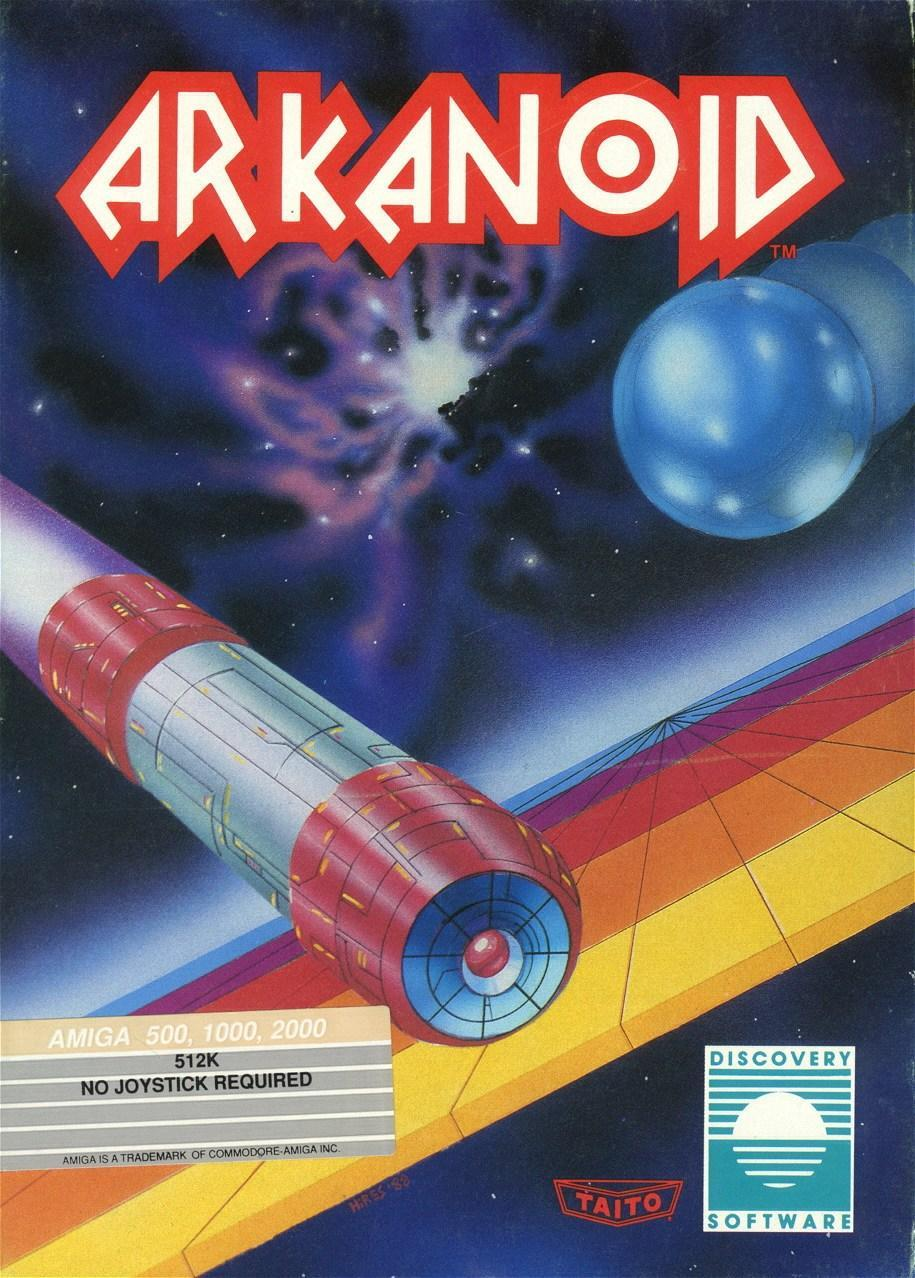
\includegraphics{images/image15.jpg}

Figura 1: Portada original Arkanoid

A lo largo del juego puede haber un gran número de variaciones que
complican el juego o que facilitan las cosas. La plataforma del jugador
puede modificar su tamaño, u obtener mejoras como disparos para romper
los bloques. La bola, puede verse modificada mediante variaciones de
tamaño o en la física del juego como romper varios bloques sin rebotar o
incluso multiplicarse. Y los bloques pueden variar en su posición e
incluso desplazarse con el fin de finalizar el juego cuando llegan
abajo.

\begin{enumerate}
\setcounter{enumi}{1}
\item
  \hyperdef{}{h.3o7alnk}{\subsection{Nuestra versión}\label{h.3o7alnk}}
\end{enumerate}

~~~~~~~~Es nuestra versión las cosas son sencillas. El usuario proviene
de defender la facultad (nave espacial tfg-III) de unos invasores, y
tras finalizar, recibirá una misión, que es la de despejar el campo de
batalla para poder despegar la nave. Para ello debe abrir paso
reciclando escombros, haciendo uso del panel de reciclaje que se sitúa
en la tercera planta, y que se accede a él, apuntando al código QR
de~Super Mario~situado junto a una de las consolas.

~~~~~~~~~~~~~~~~~ ~~~~~~~~~~~~~~~~~


\includegraphics{images/image14.jpg}

Figura 2: qr Super Mario

Una vez se reconozca el ImageTarget (el QR de Super Mario), aparecerá un
viejo televisor, y en su pantalla se observa el juego y dos contadores.
El objetivo es sencillo, hay que despejar los escombros. Hay un minuto
para realizar dicha tarea o hasta que la bola atraviese la deathzone.
Cuantos más residuos recicle, mayor será la puntuación que arrastrará al
siguiente juego.

Una vez en situación, mientras enfoca al target para no perder de vista
la escena, el jugador deberá arrastrar su dedo por la pantalla de su
smartphone para poder desplazar la plataforma y controlar donde rebota
la bola. Mientras hace eso, la bola irá rebotando y el tiempo
decrementando. A medida que destruya objetivos, la puntuación crecerá y
el tiempo se irá agotando.

{[}captura del juego enfocado en el museo de la facultad{]}

El juego está ambientado en un entorno espacial, haciendo referencia al
hilo del juego pero solo de forma superficial. Lo que conforma el tema
del espacio es lo que aparece en la pantalla del televisor que contiene
la escena. Pero, en realidad, la escena tiene una connotación~retro,
donde un antiguo televisor al lado de una de las consolas que en un
pasado ejecutaba el juego, quiere recrear la forma primitiva de jugar al
Arkanoid;~en un televisor de tubo~y con un juego sencillo que era para
lo que daba de sí la tecnología y los medios de la época.

Con esta recreación, lo que se intenta es, no tanto simular un juego
entretenido para cumplir con el objetivo de la historia, si no el
recrear una escena pasada basada en este juego. De esta forma, se hace
uso de la RA en este caso, no como medio de entretenimiento a través las
mecánicas que proporciona, si no generando una escena para mejorar la
experiencia del visitante del lugar, el museo de la facultad.

~~~~~~~~

\begin{enumerate}
\setcounter{enumi}{2}
\item
  \hyperdef{}{h.23ckvvd}{\subsection{Implementación}\label{h.23ckvvd}}
\end{enumerate}

\hyperdef{}{h.ihv636}{\paragraph{Diseño}\label{h.ihv636}}

~ ~ ~ ~ La escena se conforma por los siguientes elementos:

\begin{itemize}
\itemsep1pt\parskip0pt\parsep0pt
\item
  ARCamera e ImageTarget como elementos principales en una escena de RA.
  La propia librería de~Vuforia~nos provee de ellos, solo hay que
  definir el Image target al que reacciona la escena y añadirlos; del
  resto ya se encarga su lógica interna.
\item
  Un modelo 3D de un televisor que hace de contenedor de la escena y que
  no tiene ninguna mecánica asociada.
\item
  La bola, en la que se han implementado dos componentes; uno físico
  para hacer que esta rebote, y un script cuya finalidad es la de
  destruir los bloques, o mejor dicho, la de lanzar la animación de
  destrucción del bloque y finalizar el juego al acabar con todos los
  bloques, o, al salirse de la zona de juego. Para evitar problemas y
  por lógica del juego, aunque la escena sea 3D los componentes sobre
  este juego son en 2D.
\end{itemize}

\begin{itemize}
\itemsep1pt\parskip0pt\parsep0pt
\item
  Ball Material: Es un material de Unity que, junto al
  componente~RigidBody2D, elimina la gravedad en el objeto, configura a
  este para poder rebotar, consigue que la fuerza aplicada sobre la bola
  sea infinita, de forma que no pare jamás de desplazarse; y, define las
  coordenadas en las que puede desplazarse el objeto (x e y) y en las
  que puede rotar (ninguna).
\end{itemize}

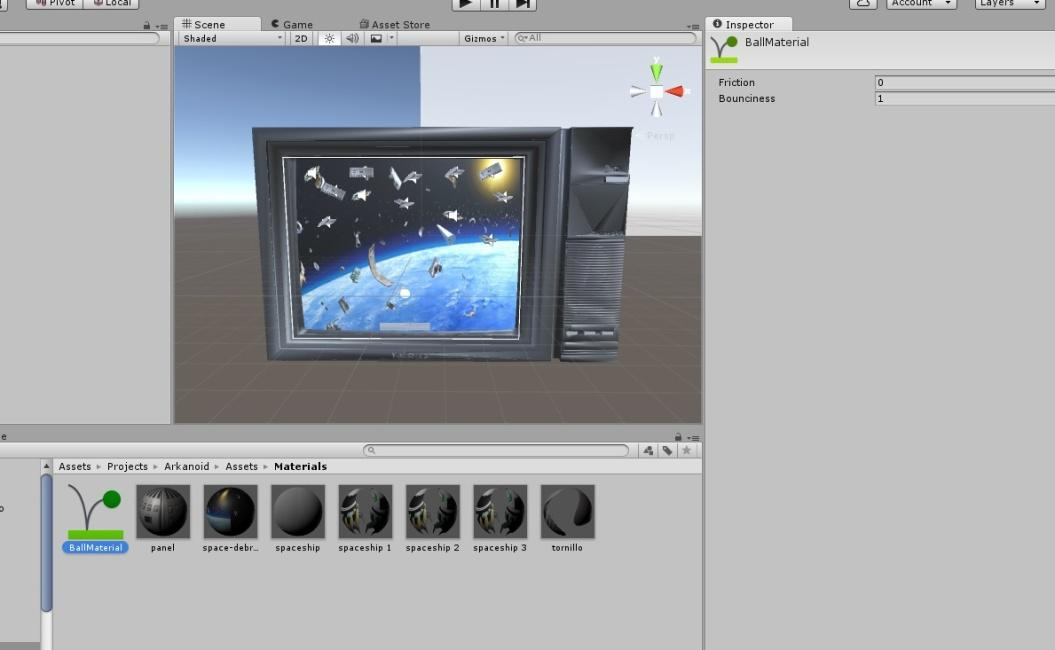
\includegraphics{images/image17.jpg}

Imagen X: BallMaterial

\begin{itemize}
\itemsep1pt\parskip0pt\parsep0pt
\item
  BoxCollider2D: Para controlar todo el tema de colisiones. En este
  caso, el Collider que envuelve a la bola es un cuadrado rotado 45
  grados para evitar problemas en los rebotes.
\end{itemize}

~~~~~~~~~~~~~~~~~ ~~~~~~~~~~~~~~~~~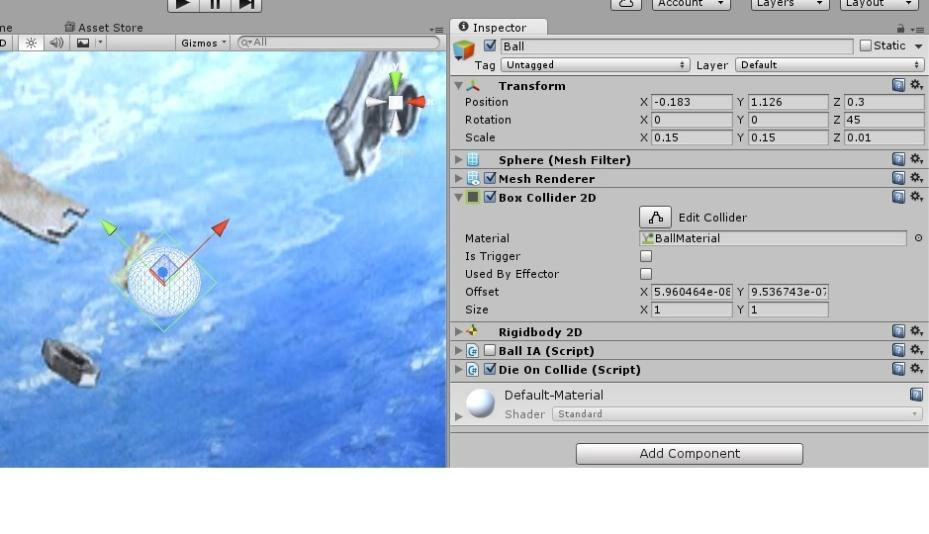
\includegraphics{images/image16.jpg}

Figura X: BoxCollider Bola Arkanoid

\begin{itemize}
\itemsep1pt\parskip0pt\parsep0pt
\item
  Los bloques, que se reparten por la escena esperando a que la bola
  colisione con ellos y recibir así, la orden de que se lance su
  animación de destrucción y se aumente el marcador.
\end{itemize}

\begin{itemize}
\itemsep1pt\parskip0pt\parsep0pt
\item
  Audio source: el componente que da sonido a la acción de destrucción.
\item
  Animación: la animación de destrucción que se lanza al colisionar con
  la bola. Esta se genera por interpolación, ya que es el sistema del
  que nos dota Unity, y lo que hace es reducir la escala del objeto a
  cero.
\end{itemize}

~~~~~~~~~~~~~~~~~ ~~~~~~~~~~~~~~~~~

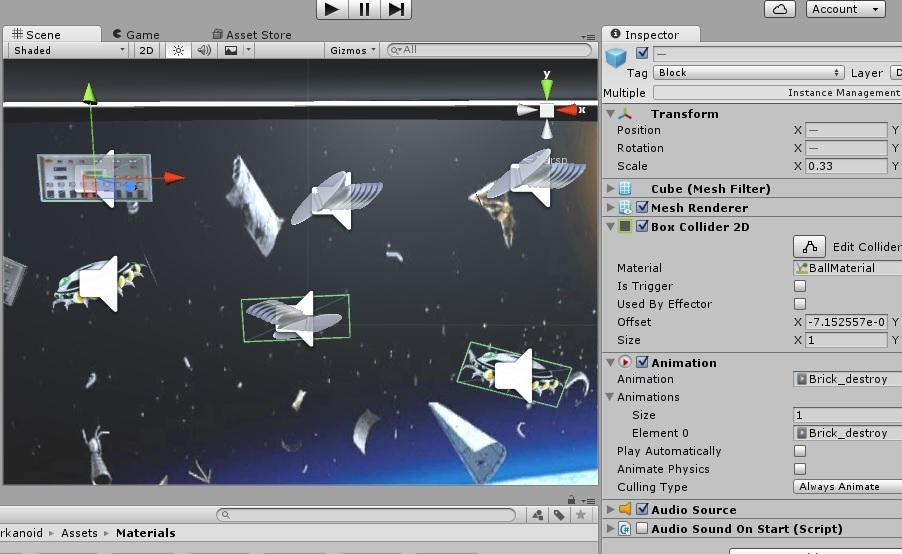
\includegraphics{images/image20.jpg}

Figura X: Distintos tipos de bloques del Arkanoid

\begin{itemize}
\itemsep1pt\parskip0pt\parsep0pt
\item
  La plataforma: Esta contiene un componente que reacciona a los eventos
  de la pantalla táctil y que le permite desplazarse, además también
  tiene un~RigidBody2D~cuyas constraints impiden que pueda verse
  desplazado en el eje vertical o rotado.
\item
  Canvas: Contiene la información del estado del juego. Este objeto y
  sus hijos, a diferencia del resto, en escena, se muestra en función a
  la pantalla del dispositivo en el que se ejecuta el juego y no en
  función de lo que enfoca la cámara. Sus hijos son, el marcador, el
  contador de tiempo y la pantalla de precarga que muestra la
  información de la ejecución del juego al usuario.
\end{itemize}

\hyperdef{}{h.32hioqz}{\paragraph{Desarrollo}\label{h.32hioqz}}

~~~~~~~~~~~~~~~~~Para el Arkanoid, se han tenido que implementar las
siguientes lógicas de juego:

\begin{enumerate}
\itemsep1pt\parskip0pt\parsep0pt
\item
  ScreenDragListener.cs:
\end{enumerate}

~~~~~~~~Se encarga de capturar las pulsaciones en pantalla. En su
método~Update ()~se comprueba con cada llamada si la pantalla ha sido
pulsada; si es así, se guarda el punto inicial donde se detectó la
pulsación y se guarda, de forma que al volverse a llamar al método, esta
vez, no solo se comprueba si ha habido contacto con la pantalla, sino
que, además, se comprueba si ha habido variación en la posición del
punto.

~~~~~~~~El script, tiene una interfaz interna. En el método~Start (), se
comprueba todos los componentes que implementan dicha interfaz en la
escena y se almacenan en un array. Cada vez que se detecta y calcula un
movimiento de~drag~sobre la pantalla del dispositivo, se recorren los
componentes del array. Estos reciben, a través del método, las
variaciones en los ejes de la pulsación; y así pueden realizar las
acciones correspondientes.

\begin{enumerate}
\setcounter{enumi}{1}
\itemsep1pt\parskip0pt\parsep0pt
\item
  BallIA.cs:
\end{enumerate}

~~~~~~~~No tiene mucha explicación, aplica una fuerza en dos coordenadas
que se le asignan como atributos en el momento en el que está activa y
se toque por primera vez la pantalla.

\begin{enumerate}
\setcounter{enumi}{2}
\itemsep1pt\parskip0pt\parsep0pt
\item
  DefaultTrackableEventHandle:
\end{enumerate}

~~~~~~~~~Es un script que viene por defecto asociado
al~ImageTarget~de~Vuforia. En este caso, hemos hecho una leve
modificación sobre este script, donde hemos añadido un array de
componentes que, cuando se detecta el QR en escena (OnTrackingFound ())
se recorre y estos se van activando.

\begin{enumerate}
\setcounter{enumi}{3}
\itemsep1pt\parskip0pt\parsep0pt
\item
  DieOnCollide.cs:
\end{enumerate}

Con dos parámetros que definen las etiquetas de los~gameObjects~que se
comportarán como enemigo (el gameObject que delimita la deathzone) y los
objetivos (los bloques que se destruyen al colisionar con ellos).
Implementa el método~OnCollisionEnter2D (), que es aquel al que llama el
collider 2D cuando entra en colisión el~gameObject~con otro objeto con
collider. Cuando se detecta una colisión, se comprueba la etiqueta del
objeto con el que se ha producido y si es de tipo enemigo, se destruye
el propio objeto y se pasa a la siguiente escena. Si es de tipo
objetivo, se llama a la animación de destrucción de este, se aumenta el
marcador y se comprueba si quedan más, para que, en el caso de que no,
pasar también a la siguiente escena.

Los mencionados son los más importantes, ya que son los que dotan de
lógica al juego, aunque existen más de los que se hacen uso como el
globalGameManager, que es el encargado de navegar entre escenas,
ScoreMarkerObserver~y TimeMarkerObserver, que pintan en el canvas el
estado del juego o un script que se añade a la escena para controlar el
back de nuestro dispositivo. Además, hay también otros scripts sencillos
que controlan el resto de los objetos de la escena.

\begin{enumerate}
\setcounter{enumi}{3}
\item
  \hyperdef{}{h.41mghml}{\subsection{Conclusiones}\label{h.41mghml}}
\end{enumerate}

~~~~~~~~La RA tiene muchos usos como se menciona en el estado del arte.
En este caso, el objetivo principal no es el de aprovecharnos de las
dinámicas que nos provee para convertirlas en objeto de entretenimiento,
si no el de dotar de dinamismo una parte del museo, ya que aportamos
información de uno de los objetos expuestos en forma de videojuego (una
versión propia que funcionaba en dicha máquina).

Una de las partes complejas en el desarrollo del juego, es la de
configurar una forma de jugar en la que se le haga posible al usuario
interaccionar con su dispositivo mientras apunta al target. Para esto se
han hecho diferentes pruebas, y se ha llegado a la configuración actual
teniendo en cuenta los siguientes factores:

\begin{itemize}
\itemsep1pt\parskip0pt\parsep0pt
\item
  El usuario~tiene una posición incómoda al utilizar su Smartphone. Él
  tiene que apuntar a la imagen mientras interacciona con el teléfono
  para evitar que la bola caiga. La mejor solución en este caso es la de
  implementar una mecánica basada en detectar el arrastre del dedo de la
  pantalla y que sea este movimiento el que desplace la plataforma en el
  juego. De esta forma, el usuario puede apuntar sin problema al QR
  mientras a su vez puede jugar. Esta forma de hacer las cosas consigue
  los dos objetivos, una mantener la cámara fijada en el target, y dos
  la de hacer cómodo junto con esto el poder manejar la plataforma.
\item
  La complejidad del juego. En este caso se implementa un juego
  sencillo, muy intuitivo y corto, porque el jugador, por la posición
  que tiene, no puede pasar mucho tiempo jugando. El juego tiene como
  máximo un minuto de duración. Y es creemos que es la apropiada ya que
  en este período se puede jugar sin cansarse y acabar el juego si se
  tiene la habilidad suficiente sin que el cansancio de la posición
  evite dicho propósito.
\item
  La escena. Es cierto que el modelo 3D del televisor no ayuda mucho a
  la jugabilidad. Pero en este caso en el que recrear una escena es casi
  más importante que la experiencia del jugador en el juego. Se ha
  preferido penalizar un poco la jugabilidad (tampoco en exceso) para
  añadir este elemento de forma que añadiendo este objeto a la escena,
  se haga una referencia a la forma de jugar de la época.
\end{itemize}

{[}imagen de un usuario apuntando al target y jugando{]}

Con este juego respecto al desarrollo de RA con~Unity~y~Vuforia, los
conceptos sintetizados son:

\begin{itemize}
\itemsep1pt\parskip0pt\parsep0pt
\item
  Aunque se trate de una escena 3D el uso de componentes 2D en los
  objetos de la escena simplifican mucho el trabajo, ya que al no tener
  que contar con un eje más; controlar el movimiento de la bola, los
  rebotes y las colisiones es más sencillo. Al fin y al cabo es como
  mantener el eje restante en un objeto 3D bloqueado pero esto lo hace
  por ti, por lo que te ahorras muchos quebraderos de cabeza a la hora
  de controlar casuísticas que se pueden escapar por ser detalles tan
  pequeños.
\item
  El manejo de los componentes~Collider~y~RigidBody~que en esta escena
  hay que modificar el material por defecto para cambiar la lógica de la
  gravedad, el rozamiento, etc.; que en este caso, no es el que está por
  defecto, ya que en este juego no hay nada de eso. Además hay que hacer
  uso de las constraints del~RigidBody~para poder bloquear las
  rotaciones y desplazamientos de algunos de los objetos de la escena
  que no interesan que puedan moverse.
\item
  La depuración del juego en modo escena en vez de hacer uso de la
  cámara. En Vuforia es normal el uso de una webcam para probar tu
  escena, pero en este caso, para probar el juego, era incómodo el tener
  que estar usando dicho elemento, por lo que, desactivando dicha opción
  de depurar la webcam en el~ImageTarget~y colocando
  la~ARCamera~apuntando a nuestro modelo 3D podíamos depurar simplemente
  haciendo click en el play del IDE de Unity sin preocuparnos de apuntar
  al QR. Lo malo de este planteamiento es que traía un problema consigo,
  los eventos de pantalla; por defecto,~Unity~no detecta como eventos de
  pantalla en un dispositivo Android el uso del ratón. Para solventar
  esto se hizo uso de una aplicación llamada~UnityRemote, que lo que
  hace es mostrar en la pantalla de nuestro dispositivo la escena que se
  está ejecutando en el IDE; y de esta forma podemos capturar los
  eventos que se realizan sobre esta pantalla.
\end{itemize}

{[}imagen del depurador de Unity y la tablet capturando la escena{]}

\begin{itemize}
\itemsep1pt\parskip0pt\parsep0pt
\item
  OnTrackingFound ()~es un método que contiene el~ImageTarget~en uno de
  sus scripts por defecto, y que en un principio, parece que se encarga
  de habilitar todos los hijos que cuelgan de él en el momento en que se
  reconoce el QR asignado. Pero no, uno de los problemas en el
  desarrollo fue, que aún sin tener enfocado el QR; aunque no se vieran
  los objetos de la escena, todos los componentes de estos, si se
  ejecutaban. Esto es, porque lo único que hace el método
  OnTrackingFound (), solo es renderizar los objetos en escena cuando se
  detecte el~ImageTarget, por lo que se modificó este método para,
  además, los scripts, que deshabilitados por defecto al comienzo de la
  escena, se habilitarán al llamarse este método.
\end{itemize}

\begin{center}\rule{3in}{0.4pt}\end{center}

Capítulo 7:

Water Pipes

\begin{enumerate}
\item
  \hyperdef{}{h.vx1227}{\subsection{Historia}\label{h.vx1227}}
\end{enumerate}

~~~~~~~~Este juego fue creado a finales de los años 80 bajo el nombre de
``Pipe Mania'' por ``The Assembly Line'', teniendo muchas versiones a lo
largo de los años. Las primeras fueron realizadas por el estudio
``LucasFilm Game'' que lanzó el juego ``Pipe Dream''.

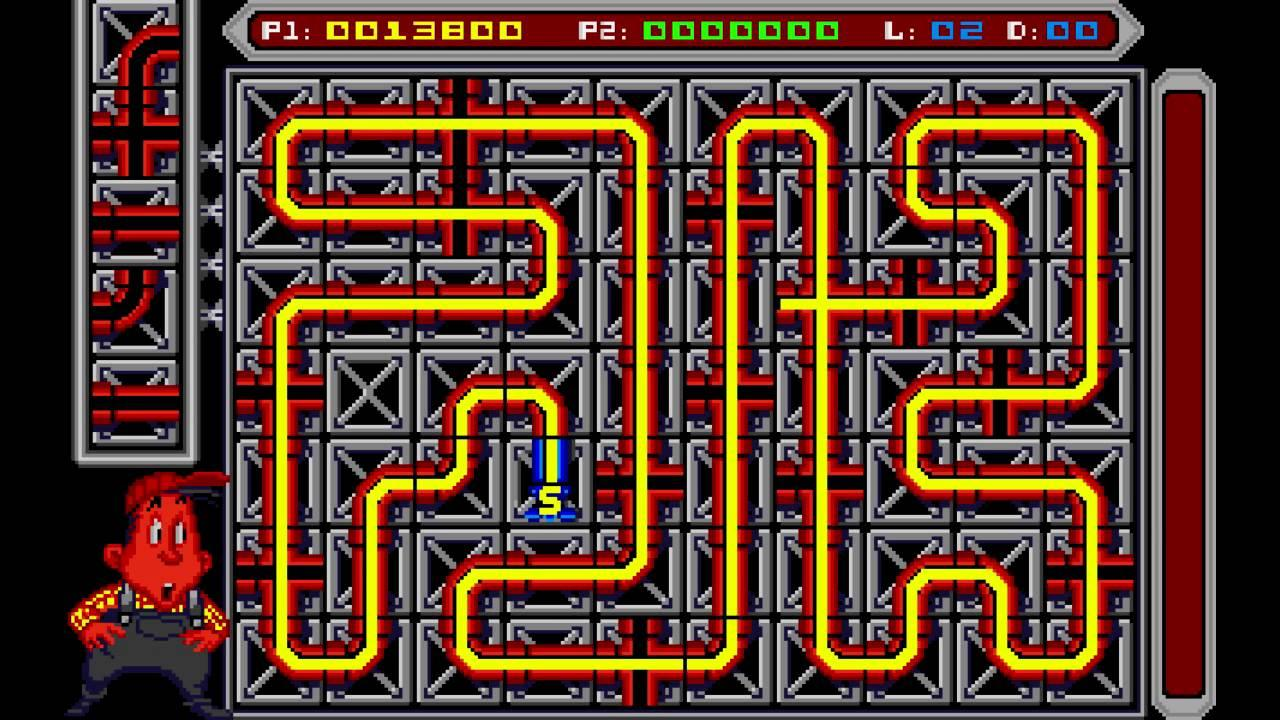
\includegraphics{images/image18.jpg}

Imagen 7.1: Juego original de 1989

Aunque posteriormente fueron lanzadas otras versiones del juego para PC,
PS2, NintendoDS y PSP.

En la versión original, el juego consistía en ir colocando las tuberías
que salían de forma aleatoria en un tablero (matriz de NxN) de tal
manera que el agua pudiera fluir por ellas. El objetivo, era construir
el mayor recorrido posible antes de que el agua lo inundara todo. Cada
tubería llena de agua sumaba puntos y cada tubería que no hubiera sido
inundada a la finalización del juego restaba puntos para obtener así la
puntuación final. En cada nivel se iban complicando las cosas, esto lo
conseguían poniendo posiciones de la matriz de juego en las cuales no se
pudieran colocar tuberías. O comenzando antes a fluir el agua por las
tuberías, dando al jugador menos tiempo de reacción.

\begin{enumerate}
\setcounter{enumi}{1}
\item
  \hyperdef{}{h.3fwokq0}{\subsection{Nuestra versión}\label{h.3fwokq0}}
\end{enumerate}

~~~~~~~~En nuestra versión del juego, existen algunas diferencias con
respecto a la versión original. La principal es la mecánica del juego ya
que en esta ocasión el usuario acaba de exterminar al enemigo que estaba
poniendo en peligro a la Facultad, y ahora su misión cambia para poder
despegar la nave y ponerse a salvo definitivamente. En esta última
misión el jugador se encontrará frente a frente con los conductos de
refrigeración de la nave, el problema es que debido a la batalla éstos
se han dispersado y si quiere despegar la nave tendrá que reordenarlos
para que el agua pueda fluir correctamente.

Al comienzo, el jugador verá una matriz rellena aleatoriamente con estos
conductos, además de una salida y una meta. Por lo tanto, el objetivo
del jugador es ir cambiando de posición las tuberías que encuentra en la
matriz, entre sí, para que el agua pueda fluir del punto de origen al de
destino. En esta ocasión, el jugador tiene 6 segundos por cada tubería
para ir colocando las demás y otros 6 segundos adicionales desde que el
juego comienza hasta que la casilla de salida comienza a llenarse. Para
poder despegar la nave, el agua ha debido fluir por todas las tuberías
necesarias para llegar a la meta. En cambio si el agua ya ha comenzado a
fluir y el jugador no ha conseguido recolocar los conductos, en cuanto
el agua no encuentre un camino factible la nave ya no se podrá despegar
y el juego terminará.

\begin{enumerate}
\setcounter{enumi}{2}
\item
  \hyperdef{}{h.1v1yuxt}{\subsection{Implementación}\label{h.1v1yuxt}}
\end{enumerate}

\hyperdef{}{h.4f1mdlm}{\paragraph{Diseño}\label{h.4f1mdlm}}

Existen dos elementos fundamentales, en cualquier aplicación de RA, y
que nos lo proporciona la librería de Vuforia, la AR Camera y el Image
Target.

\begin{itemize}
\itemsep1pt\parskip0pt\parsep0pt
\item
  AR Camera: Es la cámara del juego, y a nivel de usuario del Unity
  funciona como ``main camera'' de otros juegos sin RA.
\item
  Image Target: Este objeto también nos lo proporciona Vuforia, y cuando
  lo configuremos con el código QR (u otra imagen o texto) será el
  responsable de relacionar la escena con lo que nuestro dispositivo
  móvil este leyendo.
\end{itemize}

Para este juego existe un solo tipo de objeto, el quad que representan a
los conductos. Todos estos objetos son hijos del Image Target.

\begin{itemize}
\itemsep1pt\parskip0pt\parsep0pt
\item
  Quad: todo el juego se compone de 25 (matriz de 5x5) objetos Quad que
  representan los conductos de refrigeración. A cada objeto se les han
  incluido los mismo componentes:
\end{itemize}

\begin{itemize}
\itemsep1pt\parskip0pt\parsep0pt
\item
  Box Collider: para detectar la colisión y así poder intercambiar dos
  objetos entre sí, en este caso, solo existe la colisión entre el
  usuario y los objetos (Touch).
\item
  RigidBody: Elimina la gravedad de los objetos y congela ciertos
  movimientos de desplazamiento y rotación de estos, en este caso hemos
  querido bloquear todas las rotaciones y la dimensión Z del
  desplazamiento. Esto es debido a que aunque es un juego en 3D, la
  experiencia con el jugador es totalmente en 2D y esos movimientos no
  nos serán necesarios.
\end{itemize}

\begin{itemize}
\itemsep1pt\parskip0pt\parsep0pt
\item
  Animación: Aunque el único objeto ``visible'' en el juego sean los
  conductos (Quad), cada uno de ellos contiene un GameObject como hijo.
  La funcionalidad de éste es la animación del agua cuando pasa por la
  tubería, por lo que cada uno de estos ``hijos'' contienen también los
  mismos componentes cada uno:
\end{itemize}

\begin{itemize}
\itemsep1pt\parskip0pt\parsep0pt
\item
  Sprite Renderer: Esto es necesario, ya que la animación se compone de
  un sprites.
\item
  Animator: que contiene el Animator Controller de ese tipo de tubería.
  Cada controlador suele tener dos animaciones por tubería, que
  dependiendo de la salida de la anterior se reproduce una animación u
  otra.
\end{itemize}

\begin{itemize}
\itemsep1pt\parskip0pt\parsep0pt
\item
  Canvas: Muestra la información del juego, en este caso se encarga de
  mostrar el tiempo restante que le queda al jugador y cuando el juego
  finaliza muestra la pantalla de marcadores, para que el jugador pueda
  introducir su nombre y así entrar en la lista de clasificados.
\item
  GameManager: Es un GameObject vacío en la escena que contiene los
  scripts para la funcionalidad del juego:
\end{itemize}

\begin{itemize}
\itemsep1pt\parskip0pt\parsep0pt
\item
  GameManagerWaterPipes: es el encargado de generar toda la escena al
  inicio del juego.
\item
  WaterController: desde este script, se controla todo el flujo del
  agua.
\item
  TimeController: clase que decrementa el tiempo de juego y el tiempo
  que tarda el agua en pasar por cada conducto.
\end{itemize}

\paragraph{Desarrollo}\label{h.2u6wntf}

~~~~~~~~Este juego se ha implementado en base al patrón command, que
encapsula la decisión de por dónde va a ir fluyendo el agua. Esta
funcionalidad es la principal de todo el juego, ya que aunque el jugador
de lo que se encarga es de intercambiar las tuberías, el objetivo del
juego es conseguir que el agua fluya desde la casilla de salida hasta la
meta.

En primer lugar, vamos a describir las clases que se encargan de las
otras funcionalidades del juego, las cuales son, el intercambio de
tuberías que realiza el jugador, la inicialización y creación del
entorno del juego y el tiempo del juego.

\begin{enumerate}
\itemsep1pt\parskip0pt\parsep0pt
\item
  TouchObject:
\end{enumerate}

Este script es el encargado de controlar el cambio de los conductos.
Para ello, lo primero que hace es capturar en el método Update todos los
toques en la pantalla y llamar a getObjectHit para obtener el objeto
presionado. Este objeto lo obtenemos a través del método
``GetNearestHitGameObject'', que genera un rayo con origen en la
ARCamera y con la dirección generada por el rayo. Y de esos se queda con
el que haya menor distancia.

Una vez tenemos el objeto presionado, tenemos que saber si ya existe
otro objeto pulsado para poder intercambiarlos, o si es el primer
elemento que queremos cambiar. Si es el primero, lo único que haremos es
cambiarle a ese objeto el tag a ``ButtonPush'' y si es el segundo,
obtenemos el que ya hemos pulsado anteriormente e intercambiamos su
posición.

\begin{enumerate}
\setcounter{enumi}{1}
\itemsep1pt\parskip0pt\parsep0pt
\item
  GameManager:~~~~~~~~
\end{enumerate}

Es el encargado de crear dinámicamente todos los objetos de la escena al
comienzo del juego, y de llevar el control del tiempo que tiene el
jugador para completar la misión. Lo primero que hace es añadir los
objetos prefabs de cada tipo de conducto (Horizontal, Vertical, Codo
Derecho Arriba, Codo Derecho Abajo, Codo Izquierdo Arriba y Codo
Izquierdo Abajo)

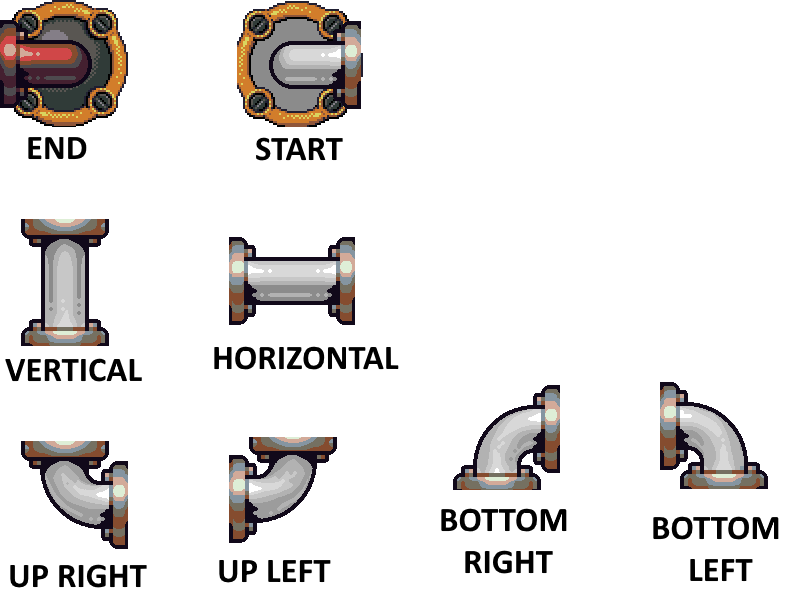
\includegraphics{images/image05.png}

Imagen 7.2: Sprites de las tuberías del juego Water Pipes

en una lista de SquareReceiver para luego ir eligiendo de manera
aleatoria los 23 conductos totales.

{[}imagen del tablero{]}

~A continuación crea la salida y la meta, ya que estos siempre van a
tener una posición fija en el tablero. Y cuando ya está todo listo, lo
único que falta es ir creando el resto del tablero. Esto lo hace
recorriendo todo el tablero desde la casilla 1 hasta la 23 y por cada
una escoge aleatoriamente un tipo de conducto, de la lista anterior.Crea
una instancia de ese tipo de objeto que será un hijo del Image Target.
Dándole además las propiedades como la posición, el nombre, y la escala.
Esta instancia la guardamos en un array del tipo SquareReceiver para
luego poder acceder a él. El método Update controla el tiempo del juego.

Por último, vamos a describir las clases necesarias para controlar el
flujo del agua.

\begin{enumerate}
\setcounter{enumi}{2}
\itemsep1pt\parskip0pt\parsep0pt
\item
  WaterController:
\end{enumerate}

Este script es, junto con el gameManagerWaterPipes, el más importante,
ya que se encarga de controlar el flujo del agua, que es la
funcionalidad básica de nuestro juego. En etse caso, el flujo de agua
funciona de la siguiente manera:

Por cada tipo de conducto el agua puede fluir en dos sentidos cada vez,
por lo tanto a partir de la entrada del agua de la casilla anterior se
calculará la casilla siguiente por la que el agua debería de fluir. Y
una vez que ya sepamos cuál~es la siguiente casilla por la que tenemos
que llevar el agua, podremos comprobar si esa casilla es válida, es
decir su entrada de agua coincide con la salida de agua anterior.

\begin{enumerate}
\setcounter{enumi}{3}
\item
  \subsection{Conclusiones~~~~~~~~
  ~~~~~~~~~~~~~~~~}\label{h.n7fwcmp2b2to}
\end{enumerate}

En este caso, el juego Water Pipes es un juego sencillo que la mayoría
de la gente conoce, por lo menos en alguna de sus versiones, y que
entretiene al usuario. Al tener varias versiones del juego fue
interesante decidir cuál era la que mejor se podía adaptar a la RA.
Quizá no es el juego que más llame la atención del usuario con respecto
a este punto, sobretodo en las primeras fases de la implementación
cuando no estaban introducidas las animaciones del agua. Pero una vez,
terminado el juego la RA hace más llamativas estas, por lo que atrae más
la atención del usuario, lo que era nuestro principal objetivo al
empezar este proyecto.

Creemos que el resultado final cumple con los objetivos, ya que se ha
implementado un juego que gracias a su sencillez y que la duración no es
demasiado larga, entretiene y capta la atención del usuario.

\begin{center}\rule{3in}{0.4pt}\end{center}

Capítulo 8:

Evaluación con usuarios

\subsection{8.1.~~~~~~~~Plan de evaluación}

\paragraph{Objetivos de la evaluación}\label{h.n54uwxdkrsbi}

~~~~~~~~Nuestros objetivos a la hora de realizar test a distintos
usuarios es detectar la mayor cantidad de fallos que nosotros mismos no
podemos ver al no ser objetivos a la hora de jugar.

~~~~~~~~Cuando se desarrolla un juego, el programador realiza distintas
pruebas durante toda la implementación. Y una vez que ha terminado el
juego, intenta jugar de varias formas posibles con la única intención de
encontrar el mayor número de errores posibles para luego solventarlos.
Pero esto, no suele ser suficiente debido a que si realiza las pruebas
la misma persona que lo ha implementado, pasará por alto muchas cosas.
Comó sabe como funciona, inconscientemente jugará bien y nunca podrá
darse cuenta de si por ejemplo el juego es intuitivo, es decir, si
aunque no sepas como funciona, esta lo suficientemente bien explicado y
diseñado para que el usuario no tenga problemas de ese tipo. Entre otras
cosas.

~~~~~~~~Creemos, que la evaluación con usuario es una fase fundamental
en cualquier aplicación. Cuantas más pruebas se realicen, la aplicación
será mejor y al usuario final le será más sencillo y le tendrá una
experiencia más satisfactoria.

~~~~~~~~

~

\paragraph{}\label{h.6ypf9b5yyx1}

\begin{center}\rule{3in}{0.4pt}\end{center}

\paragraph{}\label{h.cy4d1kd5brdq}

\paragraph{Tareas a realizar}\label{h.9dug8ado9iqg}

~~~~~~~~Una vez hemos tenido una versión terminada de todos los juegos y
unidos ellos entre sí mediante una pequeña historia, damos por
finalizada la primera versión estable de nuestro juego.

Con esta versión, decidimos realizar pruebas con usuarios para mejorar
los posibles errores ~o mejorar la usabilidad de los juegos de cara a
una segunda iteración.

Al ser una aplicación, decidimos utilizar el cuestionario SUS para
realizar estas pruebas. Pero este cuestionario está en un principio
dirigido a evaluar una aplicación web, por lo que tuvimos que modificar
un poco las preguntas para adaptarlo a un juego.

La siguiente tabla muestra las preguntas finales, con las respuestas
necesarias para sacar el 100\% de la puntuación.

\begin{longtable}[c]{@{}lll@{}}
\toprule\addlinespace
\begin{minipage}[t]{0.30\columnwidth}\raggedright
N

Preguntas

Puntuación
\end{minipage} & \begin{minipage}[t]{0.30\columnwidth}\raggedright
1

Me gustaría volver a jugar

5
\end{minipage} & \begin{minipage}[t]{0.30\columnwidth}\raggedright
2

El juego tiene una complejidad innecesaria

1
\end{minipage}
\\\addlinespace
\bottomrule
\end{longtable}

Imagen 8.1: Tabla del cuestionario SUS

Una de las ventajas de este cuestionario, es que las preguntas son
sencillas y fáciles de entender. Pero también, es muy importante que es
muy sencillo de contestar ya que el usuario solo tendrá que evaluar cada
pregunta en un intervalo del 1 al 5, siendo 1 la respuesta elegida si
está muy en desacuerdo con lo que le preguntan o 5 en el caso de que
este muy de acuerdo y pudiendo valorar cualquier puntuación entre ese
intervalo del 1 al 5.

\subsection{8.2.~~~~~~~~Descripción de la metodología del análisis de
los datos}\label{h.2muw05ic1bu9}

~~~~~~~~Esta etapa del proyecto es una de las más importantes, y por eso
creemos que es necesario hacer todos los pasos necesarios para poder
sacar el mayor beneficio a estas pruebas. Decidimos reunirnos para
determinar cuáles iban a ser los pasos a seguir para conseguir la mayor
información posible.

Dividimos en varias fases este proceso, con la intención de simplificar
cada una de ellas y así tener muy claro lo que debíamos hacer en cada
momento para que no se nos escapará ningún detalle, obteniendo así, no
el mejor resultado en los test, sino lo más importante datos e
información relevante para poder mejorar nuestra aplicación

8.2.1.~~~~~~~~Primera fase

Lo primero que hicimos, una vez adaptamos las preguntas del cuestionario
a las de un juego, fue decidir sobre qué nos deberíamos fijar más
detenidamente mientras realizamos los test y así poder tomar notas sobre
ello para más tarde poder añadirlo a la evaluación final, ya que cuanta
más información se obtenga de los test a los usuarios, más mejoras
podremos realizar en nuestro juego.

Cuando tuvimos claro todos estos puntos, empezamos a realizar test a la
mayor cantidad de usuarios posibles, sin importarnos su edad, su
habilidad a la hora de utilizar un smartphone o si habían probado
previamente los juegos que hemos implementado.

8.2.2.~~~~~~~~Segunda fase

~~~~~~~~El siguiente paso, es la evaluación directa con los usuarios.
Nuestro procedimiento a seguir en esta fase, es la de que el usuario
juegue al juego y sin explicarle nada del juego previamente. Mientras el
usuario está jugando, nosotros tomamos notas que nos sirven de ayuda. Y
una vez el usuario ha finalizado el juego, se le pasa el cuestionario
para que responda a las preguntas. Por último, y aunque el cuestionario
es anónimo, le pedimos al usuario que nos anote su edad.

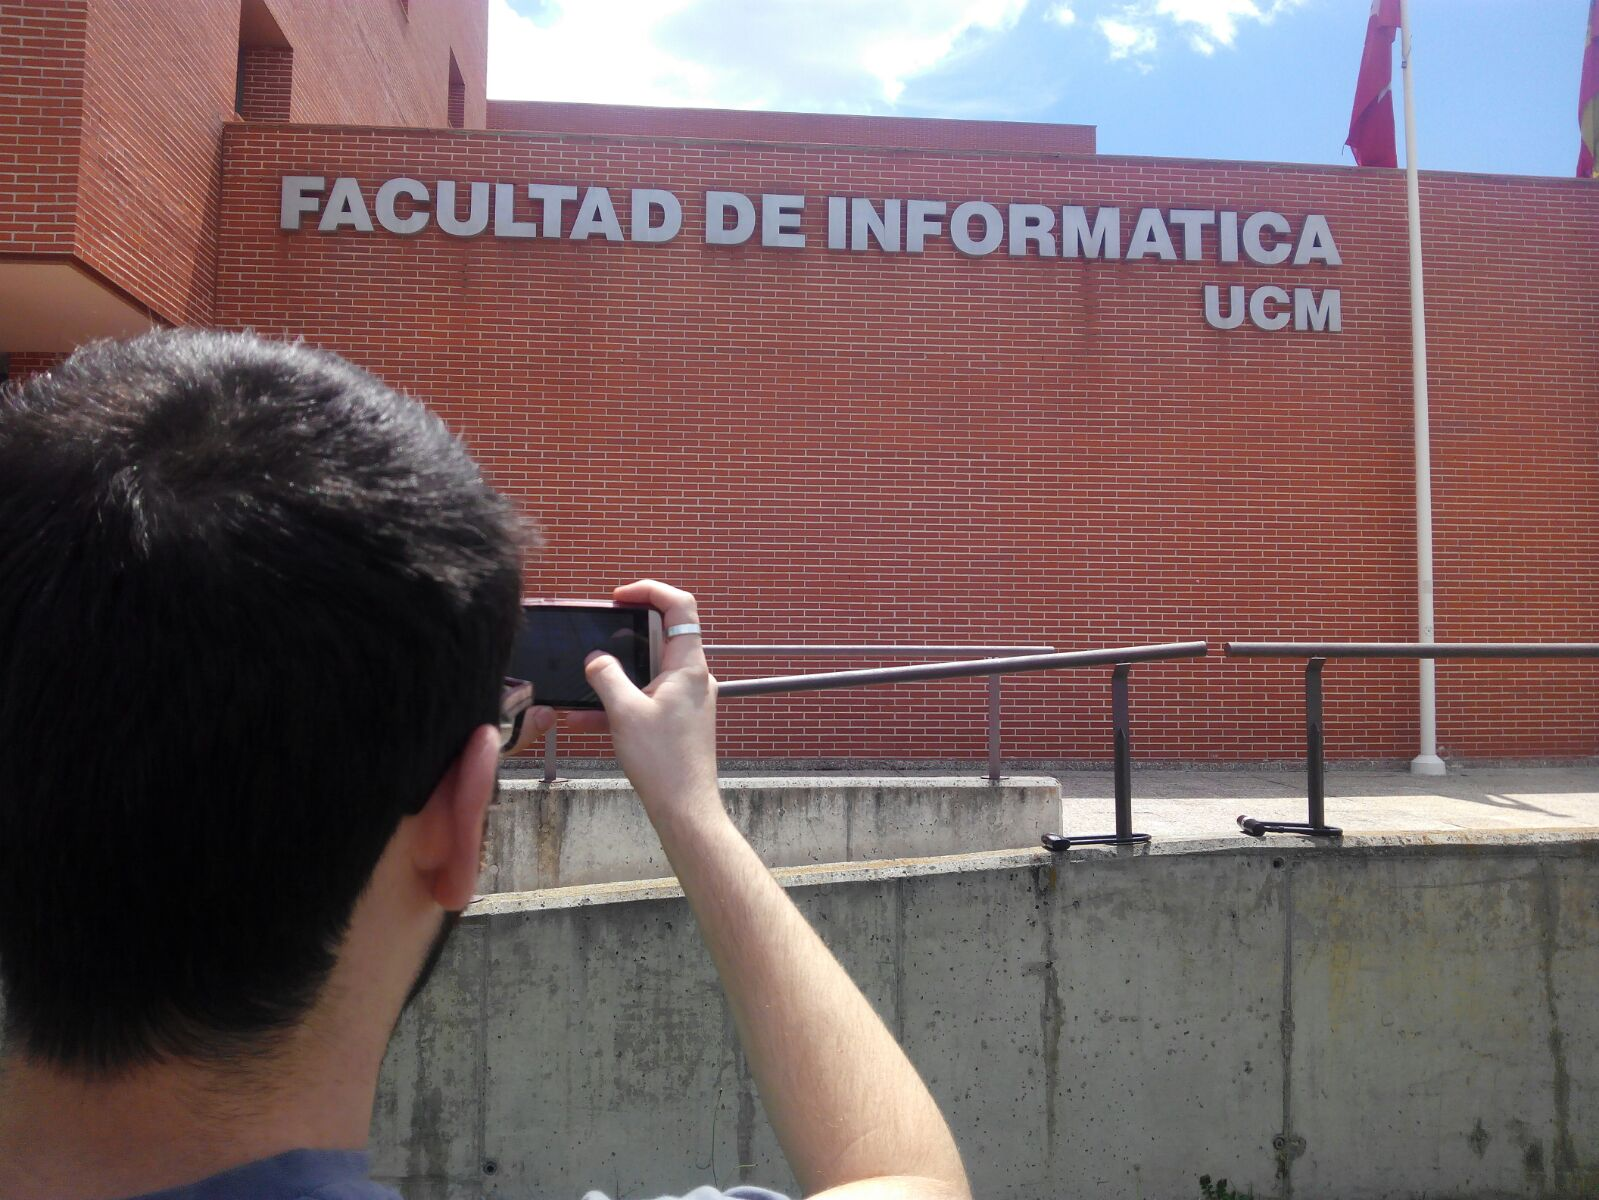
\includegraphics{images/image04.jpg}

Imagen 8.2: Usuario realizando un prueba del Space Invaders

8.2.3. Tercera fase

~~~~~~~~Con todos los cuestionarios realizados, metemos los resultados
en el excel que hemos preparado previamente con la fórmula del SUS.

Cuestionario 1

Edad 19

Space Invaders

Arkanoid

Water Pipes

5

1

4

1

3

3

5

1

2

1

1

1

1

4

3

1

2

1

5

3

3

1

4

1

5

3

3

1

1

1

90

52,5

70

~~~~~~~~Imagen 8.3: Ejemplo de resultados del cuestionario realizado a
un usuario

8.2.4.~~~~~~~~Cuarta fase

~~~~~~~~Analizamos los resultados, tanto los obtenidos a través del
cuestionario SUS, como de las notas recogidas durante la prueba del
juego.

\subsection{8.3.~~~~~~~~Primera evaluación con
usuarios}\label{h.9atqj49we7v2}

En esta primera evaluación, efectuamos un total de 14 pruebas a los
usuarios, de las cuales 7 se realizaron en la facultad y el resto desde
casa. De las que se realizaron en la facultad, todavía ningún usuario ha
realizado el cuestionario, completando el juego por el MIGS, debido a
que no teníamos instalados aún los QR necesarios para el juego.

~~~~~~~~Pese a esto, los resultados fueron de gran ayuda, y nos
permitieron hacer varias mejoras en la aplicación que aunque no eran
grandes cambios, podrían ayudar bastante al usuario a la hora de
comprender el funcionamiento del juego más rápidamente.

8.3.1.~~~~~~~~Informe de resultados

Cuestionario SUS

~~~~~~~~El análisis de resultados de la primera evaluación con usuarios,
fue muy revelador con respecto a los controles del usuario con los
distintos juegos. Tanto como los resultados del cuestionario SUS, como
los comentarios de los usuarios unidos con nuestras notas tomadas
mientras jugaban, nos revelaron que en los dos últimos minijuegos de la
aplicación era necesario realizar alguna modificación para que el
usuario pudiera manejar los controles del juego de manera más efectiva.

~~~~~~~~Es importante saber que el cuestionario SUS coloca el resultado
obtenido en un intervalo de puntuación que determina la usabilidad de la
aplicación y en nuestro caso de los mini juegos.

~~~~~~~~Este intervalo es el siguiente:

\begin{itemize}
\itemsep1pt\parskip0pt\parsep0pt
\item
  Puntuación \textgreater{} 80.3 → Buena usabilidad
\item
  80.3 \textgreater{}= Puntuación \textgreater{} 68 → Bien, pero se
  puede mejorar
\item
  Puntuación ~\textless{}= 51 → La usabilidad no es buena
\end{itemize}

A continuación mostramos el promedio de los resultados obtenidos de los
cuestionarios realizados en este primer análisis.

~~~~~~~~

Promedio primera evaluación

Space Invaders

Arkanoid

Water Pipes

78,2

52,5

55,5

Imagen 8.4: Tabla del cuestionario SUS

Simplemente con estos datos, se puede ver a primera vista lo comentado
anteriormente. El primer mini juego, según la escala SUS, no obtiene la
puntuación necesaria para obtener una buena usabilidad, pero se acerca
mucho, lo que nos indica que aunque existen ciertas cosas se pueden
mejorar, el usuario piensa que el juego tiene lo necesario para ser
jugado sin problemas y a demás que el juego le resulta entretenido.

En cambio, la puntuación de los otros dos juegos se encuentran en el
caso opuesto. Aunque no llegan a obtener el 51. límite para que la
usabilidad del juego no sea buena, se aproximan demasiado.

~~~~~~~~Información recogida de los usuarios

Los resultados del SUS, nos resultan muy útiles para obtener una visión
clara de la usabilidad de cada juego, y aunque si analizamos las
respuestas más detenidamente, podríamos hacernos una idea de los fallos
y los deseos de los usuarios. Nos es imprescindible también tomar nota,
tanto de los comentarios de los usuarios antes, durante y después de
haber probado el juego, como de las observaciones que nosotros mismos
realizamos.

En la primera evaluación, esta información es muy relevante, debido
también a que se repite las mismas opiniones o muy parecidas, en la
mayoría de los usuarios evaluados.

En las siguientes líneas mostramos las opiniones más frecuentes y
relevantes de los usuarios, por cada uno de los juegos en esta primera
evaluación.

\begin{itemize}
\itemsep1pt\parskip0pt\parsep0pt
\item
  SPACE INVADERS
\end{itemize}

\begin{enumerate}
\itemsep1pt\parskip0pt\parsep0pt
\item
  El juego sale muy pequeño con respecto al Image Target.
\end{enumerate}

\begin{enumerate}
\setcounter{enumi}{1}
\itemsep1pt\parskip0pt\parsep0pt
\item
  La dificultad del juego es demasiado sencilla.
\end{enumerate}

\begin{itemize}
\itemsep1pt\parskip0pt\parsep0pt
\item
  ARKANOID
\end{itemize}

\begin{enumerate}
\itemsep1pt\parskip0pt\parsep0pt
\item
  El control del juego, es demasiado complicado. La mayoría de los
  usuarios, no han sido capaces de controlar la barra para mantener la
  pelota a salvo.
\end{enumerate}

\begin{enumerate}
\setcounter{enumi}{1}
\itemsep1pt\parskip0pt\parsep0pt
\item
  La velocidad de la pelota es demasiado rápida, lo que hace que el
  juego sea demasiado difícil de completar con éxito.
\end{enumerate}

\begin{enumerate}
\setcounter{enumi}{2}
\itemsep1pt\parskip0pt\parsep0pt
\item
  La escena es demasiado grande, lo que obliga al usuario a separarse
  mucho del QR.
\end{enumerate}

\begin{itemize}
\itemsep1pt\parskip0pt\parsep0pt
\item
  WATER PIPES
\end{itemize}

\begin{enumerate}
\itemsep1pt\parskip0pt\parsep0pt
\item
  La mayoría de los usuarios no saben cómo controlar el juego.
\end{enumerate}

\begin{enumerate}
\setcounter{enumi}{1}
\itemsep1pt\parskip0pt\parsep0pt
\item
  El tiempo de comienzo antes de que el agua empiece a pasar por las
  tuberías es demasiado corto, por lo que los usuarios pierden antes de
  poder comprender el funcionamiento del juego.
\end{enumerate}

\begin{enumerate}
\setcounter{enumi}{2}
\itemsep1pt\parskip0pt\parsep0pt
\item
  Las casillas de Start y End, se confunden por lo que el usuario no
  sabe dónde tiene que empezar a colocar las tuberías antes de que el
  tiempo acabe.
\end{enumerate}

\begin{center}\rule{3in}{0.4pt}\end{center}

Capítulo 9:

Conclusiones y trabajo futuro

~~~~~~~~En este capítulo haremos un análisis del trabajo realizado, así
como de las decisiones que hemos tomado y los resultados de esas
decisiones.

Además, haremos un análisis de posibles trabajos futuros a partir de
éste proyecto.

\subsection{~~~~~~~~9.1.~~~~~~~~Conclusiones}

Como ya hemos comentado en el capítulo 2, la realidad aumentada tiene
unas posibilidades enormes en multitud de campos. Desde los puramente
lúdicos, como los videojuegos, hasta aplicaciones en ciencia o
educativas (como pretende ser éste trabajo). En el campo que nos ocupa,
que es la educación, encontramos infinidad de posibilidades. Desde
atraer a gente a un museo para divulgar la información de éste, hasta
formar a profesionales de la medicina con modelos en tres dimensiones de
órganos o a ingenieros para ver cómo funcionan motores, engranajes o
sistemas de transmisión en tiempo real.

~~~~~~~~Éste trabajo nos ha hecho darnos cuenta del hecho de que
probablemente, si no lo es ya, la siguiente gran revolución en los
museos sea la RA. Aporta una cantidad de posibilidades para atraer al
público que todavía, creemos, no nos podemos hacer a la idea.

~~~~~~~~Aplicaciones como ésta en los museos, con una~yincana, creemos
es muy atractiva. Ya que se consigue que el usuario vaya a distintos
puntos del museo y realice acciones determinadas, por lo que podemos
acercar contenidos del museo que quizá no fueran en apariencia tan
atractivos para los usuarios.

~~~~~~~~Teniendo esto presente, el objetivo de este proyecto era crear
un atractivo para los usuarios del museo a través de la RA y videojuegos
más que transmitir información al usuario sobre el contenido del museo.
Consideramos que esto lo hemos conseguido. Hemos creado tres minijuegos
de una dificultad muy aceptable, cada uno utilizando una manera de
interactuar por parte del usuario. Además, se puede realizar el circuito
en poco tiempo, y como se obtiene al final una puntuación que podemos
comparar con las de otros usuarios, esto dinamiza la experiencia.

\hyperdef{}{h.111kx3o}{\subsection{~~~~~~~~9.2.~~~~~~~~Líneas
futuras}\label{h.111kx3o}}

~~~~~~~~La verdad es que las posibles líneas futuras son muchísimas.
Durante el desarrollo del proyecto hemos tenido muchas ideas que no
hemos podido llevar a cabo por falta de tiempo.

~~~~~~~~Por un lado, con añadir más minijuegos o más niveles a los ya
existentes, se podría hacer otra aplicación nueva. También hemos tenido
otras ideas de minijuegos. Por ejemplo, un juego al estilo ``aplasta
topos'' de las ferias se podría poner en un cuadro informativo que hay
con imágenes de disquetes. Otro juego, más complejo, que se nos había
ocurrido era, de alguna forma, hacer que el jugador tuviera que conectar
diferentes salidas y entradas de cables en uno de los primeros
ordenadores que hay en el museo.

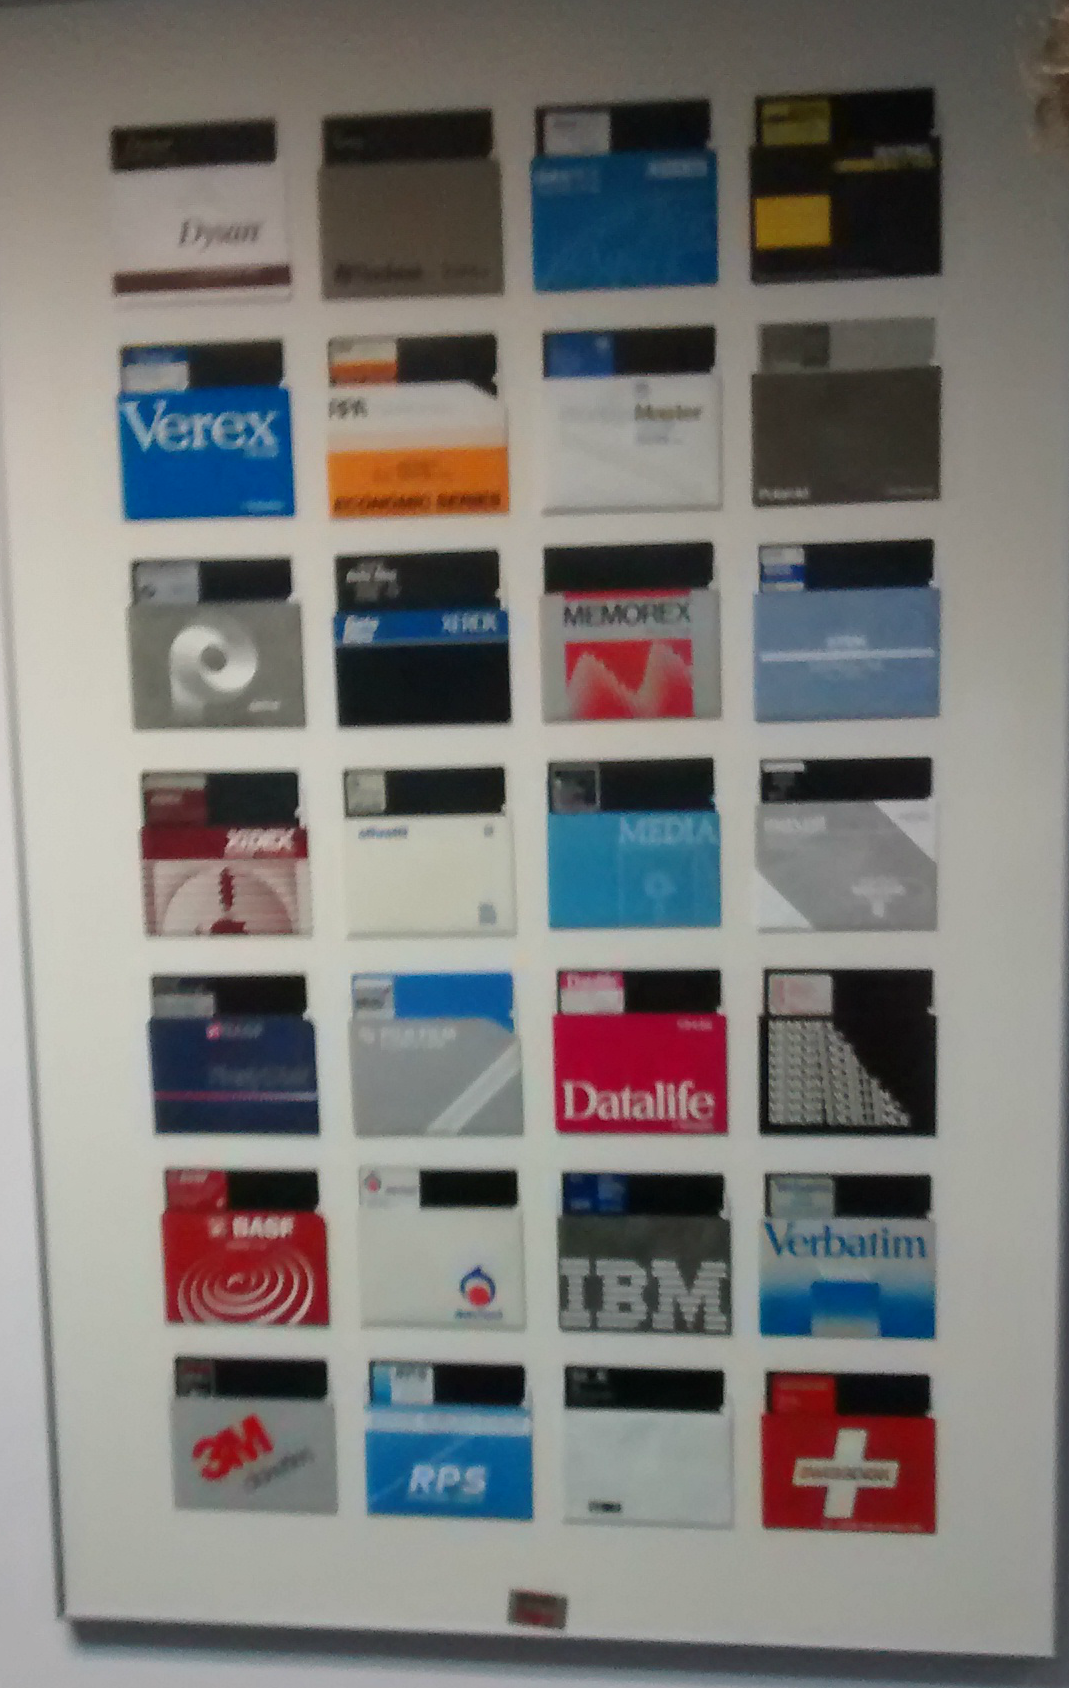
\includegraphics{images/image09.png}

Imágen 9.1: Fotografía del cuadro informativo con los disquetes

~~~~~~~~Otra posibilidad es mostrar información acerca de los equipos
expuestos y después hacer un test con preguntas al jugador.

\begin{center}\rule{3in}{0.4pt}\end{center}

\hyperdef{}{h.3l18frh}{\section{Capítulo 10:~}\label{h.3l18frh}}

Aportaciones individuales

\subsection{10.1.~~~~~~~~Organización general del proyecto}

~~~~~~~~En general nos hemos organizado de manera independiente. Cada
uno de los miembros ha realizado uno de los minijuegos, aunque luego
hemos desarrollado algunas funcionalidades juntos y otras, a parte del
minijuego de cada uno, también de manera individual. Aun siendo cada uno
de los minijuegos responsabilidad de uno de los miembros del equipo, nos
hemos apoyado cuando teníamos problemas en el desarrollo individual de
cada uno.

\subsection{10.2.~~~~~~~~Raúl Cobos}\label{h.4k668n3}

\begin{itemize}
\itemsep1pt\parskip0pt\parsep0pt
\item
  Realización de tutoriales en Unity3D para comprender en profundidad
  cómo funcionan sus escenas y sus mecánicas.
\item
  Autoaprendizaje e investigación de nuevas tecnologías para mi como era
  Vuforia.
\item
  Realización de prototipos de Unity3D y Vuforia.
\item
  Testeo con Álvar de diferentes maneras de interactuar con la RA en los
  primeros momentos.
\item
  Comunicación y reuniones con nuestro tutor Guillermo a través de
  reuniones presenciales y correos electrónicos.
\item
  Evaluación con usuarios e interpretación de éstas.
\item
  Escritura de todos los apartados de la memoria (menos los de los
  minijuegos de mis compañeros) y revisión de los contenidos del a
  misma.
\item
  Toma de decisiones con el resto de mis compañeros.
\end{itemize}

\subsection{10.3.~~~~~~~~Álvar D. Soler}\label{h.2zbgiuw}

~~~~~~~~El minijuego que yo he desarrollado ha sido el Space Invader.
Además de todo este minijuego, he llevado a cabo las siguientes tareas:

\begin{itemize}
\itemsep1pt\parskip0pt\parsep0pt
\item
  Realización de tutoriales en Unity3D para comprender en profundidad
  cómo funcionan sus escenas y sus mecánicas.
\item
  Autoaprendizaje e investigación de nuevas tecnologías para mi como era
  Vuforia.
\item
  Realización de prototipos de Unity3D y Vuforia.
\item
  Puesta en práctica de reconocimiento de texto propio en castellano.
\item
  Testeo con Raúl de diferentes maneras de interactuar con la RA en los
  primeros momentos.
\item
  Realización de fotografías en el museo para poder orientarnos cuando
  trabajáramos en nuestras casas.
\item
  Comunicación y reuniones con nuestro tutor Guillermo a través de
  reuniones presenciales y correos electrónicos.
\item
  Testeo para calibrar bien el tamaño de los Invaders y las Defensas con
  el cartel del exterior de la Facultad.
\item
  Evaluación con usuarios e interpretación de éstas.
\item
  Búsqueda de imágenes que fueran fáciles de reconocer por la cámara de
  Vuforia.
\item
  Escritura de todos los apartados de la memoria (menos los de los
  minijuegos de mis compañeros) y revisión de los contenidos del a
  misma.
\item
  Toma de decisiones con el resto de mis compañeros.
\item
  Traducción al inglés de los apartados de la memoria que están
  traducidos.
\end{itemize}

\begin{center}\rule{3in}{0.4pt}\end{center}

\hyperdef{}{h.1egqt2p}{\subsection{10.4.~~~~~~~~María
Picado}\label{h.1egqt2p}}

~~~~~~~~~~~~~~~~En mi caso, mi trabajo ha estado dividido en varias
etapas, en cada una de las cuales me he dedicado a diferentes tareas.

\begin{itemize}
\itemsep1pt\parskip0pt\parsep0pt
\item
  La primera de ellas, fue junto a mis compañeros la realización de
  tutoriales en Unity3D para comprender y afianzar los conocimientos
  sobre el funcionamiento de esta herramienta.
\end{itemize}

\begin{itemize}
\itemsep1pt\parskip0pt\parsep0pt
\item
  Como ya dijimos anteriormente, aunque si conocíamos Unity, Vuforia era
  completamente desconocida para nosotros, con lo que mi siguiente tarea
  fue la de investigación y autoaprendizaje~para conocer el
  funcionamiento de Vuforia. Y más adelante comencé con la creación de
  pequeños prototipos en Unity3d y Vuforia.
\end{itemize}

\begin{itemize}
\itemsep1pt\parskip0pt\parsep0pt
\item
  Durante todo el proceso de creación del proyecto, hemos mantenido los
  tres reuniones periódicas con nuestro director del TFG para ir
  mostrándole los avances y ponernos nuevos objetivos de cara a la
  siguiente reunión.
\end{itemize}

\begin{itemize}
\itemsep1pt\parskip0pt\parsep0pt
\item
  Una vez adquirimos los suficientes conocimientos para poder
  desenvolvernos tanto con Unity como con Vuforia, decidimos reunirnos
  los tres para diseñar el videojuego y decidir qué~minijuegos
  implementaremos.
\end{itemize}

\begin{itemize}
\itemsep1pt\parskip0pt\parsep0pt
\item
  En esa reunión, una de las decisiones que tomamos fue la de que juegos
  íbamos a implementar cada uno, y a partir de ese momento me centré~en
  la realización del minijuego Water Pipes.
\end{itemize}

Lo primero que hice fue documentarme del juego original para ver cómo
sería la mejor manera de adaptarlo a la RA.

Una de las cosas más importantes para que el juego se pudiera adaptar a
la RA, era obtener la forma de que el usuario pudiera manipular las
tuberías. Al ser una aplicación móvil, lo primero que intenté fue el
``DRAG AND DROP'', para que el jugador pulsara una tubería y la
arrastrarse~hasta donde quisiera cambiarla y al soltarla se
cambiará~automáticamente~una tubería por la otra. Pero esta opción me
dio bastantes problemas y entonces decidí que la forma en que se fueran
colocando las tuberías fuera el intercambio entre ellas, pulsando sobre
una e intercambiando por la siguiente en ser pulsada.

Una vez implementada la funcionalidad para colocar las tuberías, comencé
a implementar la parte más importante del juego; el flujo del agua. Como
existen 6 opciones de tuberías distintas y cada una de ellas tiene otras
dos direcciones posibles por las que puede circular el agua. Tenía que
buscar una forma de encapsular esa información para que lo único que nos
preocupase fuera la salida de la tubería actual y la entrada de la
siguiente. Por eso decidí usar el patrón de diseño Command.

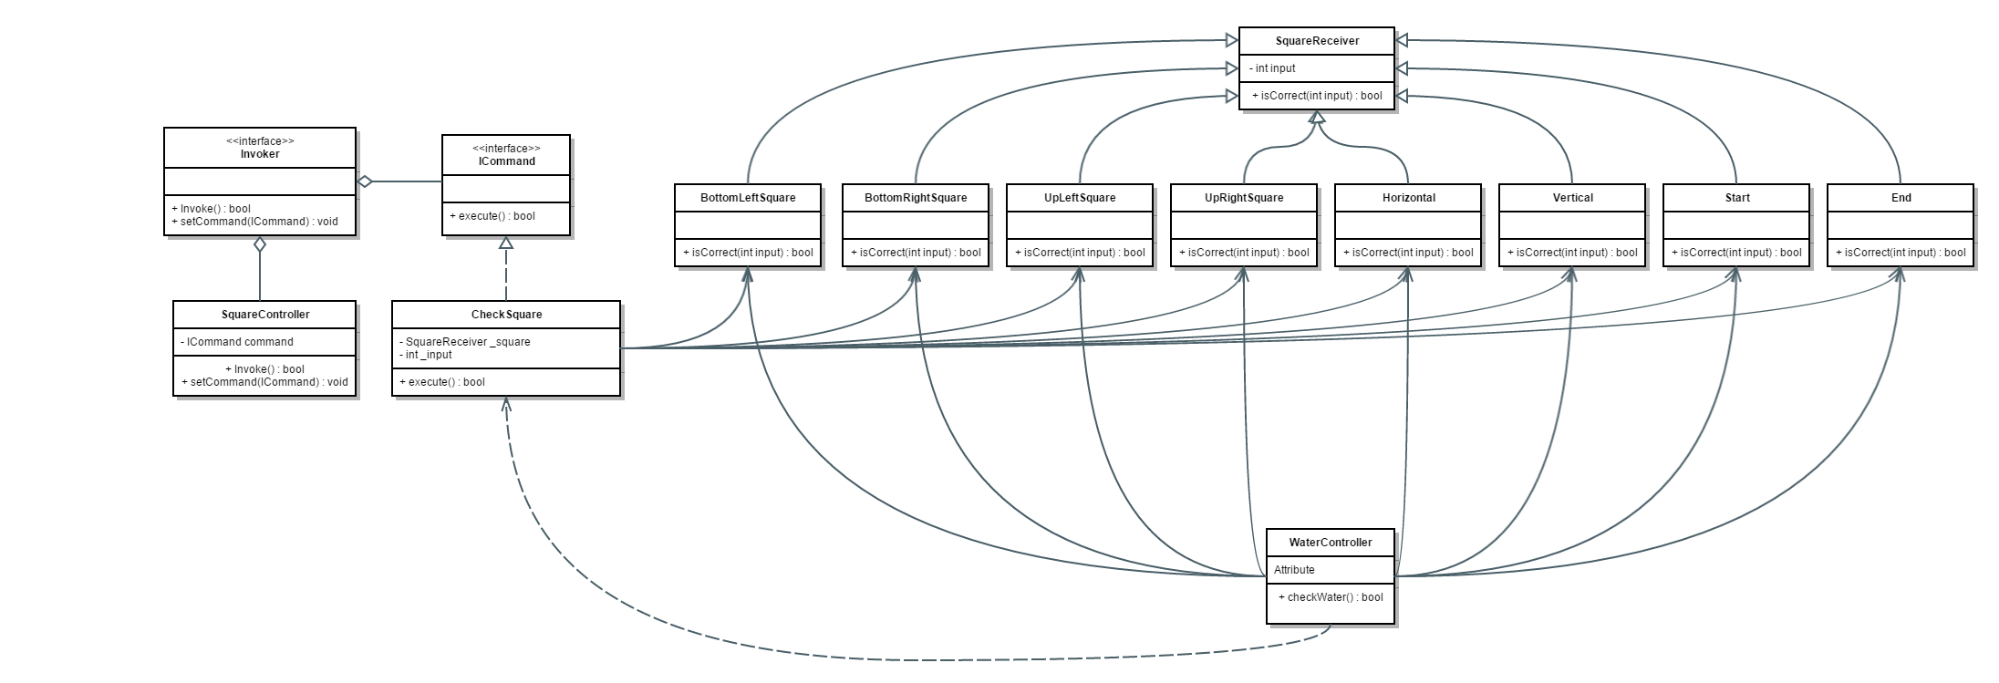
\includegraphics{images/image06.png}

Imagen 10.1: Diagrama de clase patrón Commad utilizado en Water Pipes

\begin{itemize}
\itemsep1pt\parskip0pt\parsep0pt
\item
  Al acabar la implementación del juego, el siguiente paso fue realizar
  el mayor número de test posibles a los usuarios. Los test los
  realizamos del juego completo, pero pedimos a los usuarios que
  puntuaron los juegos de manera independiente. Por eso, un vez que
  obtuvimos los primeros resultados, me dispuse a modificar el juego
  para implementar las mejoras que me aconsejaron los usuarios.
\end{itemize}

\begin{itemize}
\itemsep1pt\parskip0pt\parsep0pt
\item
  Durante todo el proyecto he colaborado en el desarrollo de esta
  memoria.
\end{itemize}

\end{document}
